\documentclass[11pt,letterpaper]{report}

\usepackage[utf8]{inputenc}
\usepackage[T1]{fontenc}
\usepackage[spanish,es-tabla]{babel}
\usepackage{lmodern}
\usepackage[scaled=0.95]{helvet}
\renewcommand{\familydefault}{\sfdefault}

\usepackage[margin=2.5cm]{geometry}
\usepackage{graphicx}
\usepackage{amsmath,amssymb}
\usepackage{booktabs}
\usepackage{array}
\usepackage{tabularx}
\usepackage{longtable}
\usepackage{enumitem}
\usepackage{fancyhdr}
\usepackage{titlesec}
\usepackage[numbers,sort&compress]{natbib}
\usepackage{xcolor}
\usepackage[hidelinks]{hyperref}

\usepackage{float} % Para usar [H] en las imágenes
\usepackage{subcaption} % Para agrupar imágenes en entornos subcaption

% Estilo de encabezados y pies de página
\pagestyle{fancy}
\fancyhf{}
\fancyhead[L]{\small\textit{Plantas de Potencia --- Energía de Biomasa}}
\fancyhead[R]{\small\thepage}
\renewcommand{\headrulewidth}{0.4pt}
\fancypagestyle{plain}{%
  \fancyhf{}
  \fancyfoot[C]{\small\thepage}
  \renewcommand{\headrulewidth}{0pt}
}

% Formato de capítulos más compacto y limpio
\titleformat{\chapter}[display]
  {\normalfont\huge\bfseries}
  {\chaptertitlename\ \thechapter}{12pt}{\Huge}
\titlespacing*{\chapter}{0pt}{-15pt}{18pt}

% Espaciado de párrafos
\setlength{\parskip}{0.45em}
\setlength{\parindent}{0pt}

\begin{document}

% -------------------------------------------------------------------------
% 1. PRESENTACIÓN (PORTADA)
% -------------------------------------------------------------------------
\input{Capitulos/00_presentacion}

% -------------------------------------------------------------------------
% 2. ÍNDICE / TABLA DE CONTENIDO
% -------------------------------------------------------------------------
\pagenumbering{roman}
\tableofcontents
\clearpage

% -------------------------------------------------------------------------
% 3. INTRODUCCIÓN (NO MÁS DE UNA PÁGINA)
% -------------------------------------------------------------------------
\pagenumbering{arabic}
\chapter*{Introducción}
\addcontentsline{toc}{chapter}{Introducción}
\markboth{Introducción}{Introducción}

La bioenergía es la fuente renovable con mayor aporte al suministro energético mundial. De acuerdo con la Asociación Mundial de la Bioenergía (WBA), en 2023 aportó aproximadamente 56~EJ de un total mundial de 622~EJ (alrededor del 9~\%); dado que las energías renovables en conjunto sumaron 92~EJ, cerca de seis de cada diez unidades de energía renovable provinieron de la biomasa \cite{wba2025gbsr}. Este predominio obedece principalmente al uso térmico (cocción, calefacción y calor de proceso industrial), diferenciándose entre el aprovechamiento tradicional de baja eficiencia y la bioenergía moderna en instalaciones industriales controladas.

En la generación eléctrica, su participación es más acotada, pero presenta un rasgo distintivo frente a la energía solar fotovoltaica y la eólica: es una fuente \textbf{despachable}, ya que el combustible puede almacenarse y la central puede generar según las necesidades del sistema eléctrico. Al cierre de 2025 la capacidad mundial instalada de bioenergía alcanzó 154~GW (cerca del 3~\% de los 5\,149~GW de capacidad renovable total), con una adición anual de 3,4~GW frente a 692~GW del conjunto de renovables \cite{irena2026capacity}. En 2024 produjo 698~TWh (7,1~\% de la electricidad renovable) con 151~GW instalados \cite{wba2025gbsr}, lo que arroja un factor de planta medio cercano al 53~\%:
\begin{equation*}
\mathrm{FP} = \frac{698\text{ TWh}}{151\text{ GW} \times 8\,760\text{ h}} = \frac{698\,000\text{ GWh}}{1\,322\,760\text{ GWh}} \approx 0{,}53
\end{equation*}

\begin{table}[h!]
\centering
\footnotesize
\caption{Indicadores globales de la bioenergía (2023--2025).}
\label{tab:biomasa_cifras}
\begin{tabularx}{\textwidth}{@{}X l l@{}}
\toprule
\textbf{Indicador} & \textbf{Valor} & \textbf{Fuente} \\
\midrule
Suministro mundial de bioenergía en Panama (2023) & 56~EJ ($\sim$9~\% total; $\sim$60~\% renovables) & \cite{wba2025gbsr} \\
Electricidad generada con bioenergía (2024) & 698~TWh (7,1~\% de la generación renovable) & \cite{wba2025gbsr} \\
Capacidad instalada de bioenergía (fin 2025) & 154~GW (+3,4~GW en 2025; +2,3~\%) & \cite{irena2026capacity} \\
Capacidad renovable total (fin 2025) & 5\,149~GW (+692~GW en 2025; +15,5~\%) & \cite{irena2026capacity} \\
Principales productores eléctricos (2024) & China: 209~TWh; Brasil: 58~TWh; EE.\,UU.: 47~TWh & \cite{wba2025gbsr} \\
Variación de costos en 2024 frente a 2023 & Costo instalado +16~\%; LCOE +13~\% & \cite{irena2025costs} \\
\bottomrule
\end{tabularx}
\end{table}

La presente monografía aborda la energía de biomasa desde la perspectiva de las plantas de potencia. El Capítulo~1 desarrolla los fundamentos fisicoquímicos, clasificación, propiedades energéticas y logística del combustible. El Capítulo~2 analiza las rutas y tecnologías de conversión: combustión directa, gasificación, pirólisis y digestión anaeróbica. El Capítulo~3 examina las escalas y configuraciones de centrales en el mundo, casos de referencia y su aporte a la estabilidad del sistema eléctrico. Finalmente, el Capítulo~4 evalúa la economía de generación, las emisiones de ciclo de vida, la captura de carbono (BECCS) y el panorama en Panamá, seguido de las conclusiones generales.

\clearpage


% -------------------------------------------------------------------------
% 4. CONTENIDO
% -------------------------------------------------------------------------
\chapter{Fundamentos de la biomasa}
\label{cap:fundamentos}

Este capítulo desarrolla las características fundamentales de la biomasa como recurso energético, desde su origen biológico y carácter renovable hasta su clasificación, propiedades fisicoquímicas, pretratamiento y logística de suministro. Se presta especial atención a los parámetros que determinan su comportamiento como combustible y que condicionan el diseño y la selección de los equipos en una planta de potencia.

\section{Concepto y carácter renovable}
\label{sec:concepto}

La biomasa se define como el conjunto de materia orgánica de origen biológico reciente (vegetal, animal o microbiano), no fosilizada, que puede aprovecharse como fuente de energía. Incluye madera, residuos forestales, cultivos energéticos, restos agrícolas, estiércol, subproductos agroindustriales y la fracción orgánica biodegradable de los residuos sólidos urbanos \cite{mckendry2002energy}. Desde el punto de vista energético, la biomasa constituye energía solar almacenada en enlaces químicos mediante la fotosíntesis, proceso por el cual los organismos vegetales capturan radiación solar y transforman dióxido de carbono y agua en compuestos orgánicos:
\begin{equation}
6\,\mathrm{CO_2} + 6\,\mathrm{H_2O} + \text{energía solar} \longrightarrow \mathrm{C_6H_{12}O_6} + 6\,\mathrm{O_2}
\end{equation}

La fotosíntesis es un proceso de baja eficiencia global: en términos generales convierte menos del 1 al 2~\% de la radiación solar incidente en biomasa. Como consecuencia, aunque el recurso es abundante a escala planetaria, presenta una baja densidad energética por unidad de superficie, lo que condiciona su recolección, transporte y aprovechamiento industrial a gran escala.

En terminología técnica, la Organización de las Naciones Unidas para la Alimentación y la Agricultura (FAO) distingue entre \textit{biocombustible} ---el portador material de energía, como leña, astillas, pellets, biogás o bioetanol--- y \textit{bioenergía} ---la energía útil obtenida a partir de dicho portador--- \cite{fao2004ubet}.

\subsection{Composición lignocelulósica}
La biomasa vegetal seca está formada fundamentalmente por tres polímeros estructurales cuyas proporciones determinan su comportamiento térmico y biológico en cada ruta de conversión \cite{mckendry2002energy}. La Tabla~\ref{tab:lignocelulosa} resume sus características principales.

\begin{table}[htbp]
\centering
\caption{Componentes estructurales de la biomasa lignocelulósica \cite{mckendry2002energy}.}
\label{tab:lignocelulosa}
\begin{tabularx}{\textwidth}{@{}l l X X@{}}
\toprule
\textbf{Componente} & \textbf{Proporción (madera)} & \textbf{Naturaleza química} & \textbf{Relevancia para la conversión} \\
\midrule
Celulosa & 40--50~\% & Polímero lineal y cristalino de glucosa & Base de la fermentación y digestión; se descompone térmicamente entre 300 y 400~\textdegree C. \\
Hemicelulosa & 20--35~\% & Polímero ramificado de diversos azúcares & Primera fracción en degradarse térmicamente (200--300~\textdegree C). \\
Lignina & 15--30~\% & Polímero aromático que aporta rigidez & Difícil de degradar biológicamente; alto poder calorífico; favorece las rutas térmicas. \\
\bottomrule
\end{tabularx}
\end{table}

\subsection{Ciclo del carbono y sostenibilidad}
Desde la perspectiva del carbono, el $\mathrm{CO_2}$ liberado durante la conversión energética de la biomasa corresponde al que la planta absorbió previamente durante su crecimiento, en una escala temporal de meses a décadas (\textit{ciclo corto del carbono}). En contraste, la combustión de combustibles fósiles libera carbono que permaneció almacenado en la corteza terrestre durante millones de años.

No obstante, la biomasa es renovable únicamente si el recurso se repone a un ritmo compatible con su consumo, sin comprometer la fertilidad del suelo ni el equilibrio de los ecosistemas. Asimismo, la neutralidad de carbono no es automática: el Grupo Intergubernamental de Expertos sobre el Cambio Climático (IPCC) señala que el balance climático real depende de las emisiones de toda la cadena de suministro (cosecha, transporte, secado, densificación), de los posibles cambios directos e indirectos en el uso del suelo y de que la tasa de extracción no supere la regeneración \cite{chum2011ipcc}. Los balances más favorables se alcanzan al valorizar residuos que de otro modo se descompondrían emitiendo metano o se quemarían a cielo abierto.

\section{Clasificación por origen}
\label{sec:clasificacion_origen}

Aunque la biomasa puede clasificarse según el reino biológico (vegetal, animal o microbiana), en ingeniería energética resulta más práctico clasificarla por fuente o sector de procedencia. El origen determina la humedad, estacionalidad, disponibilidad geográfica, contenido de cenizas y logística de recolección, condicionando directamente la tecnología de conversión \cite{irena2023residues}.

\begin{table}[htbp]
\centering
\small
\caption{Clasificación de la biomasa según su origen y sector de procedencia.}
\label{tab:clasificacion_origen}
\begin{tabularx}{\textwidth}{@{}p{2.6cm} X p{2.7cm} X@{}}
\toprule
\textbf{Categoría} & \textbf{Ejemplos representativos} & \textbf{Ruta típica} & \textbf{Consideraciones de ingeniería} \\
\midrule
Residuos agrícolas & Paja y cascarilla de arroz, rastrojo de maíz, restos de poda & Combustión, gasificación & Estacionales y dispersos; la cascarilla de arroz presenta elevado contenido de cenizas (sílice). \\
Residuos agroindustriales & Bagazo de caña, cascarilla de café, cáscara de coco, raquis de palma, efluentes & Combustión en calderas (CHP); digestión de efluentes & Concentrados en planta industrial, sin costo adicional de recolección. El bagazo representa $\sim$30~\% de la caña molida \cite{er2019centroamerica}. \\
Residuos forestales y madereros & Ramas, corteza, aserrín, astillas, licor negro & Combustión, pellets, gasificación & Base de las grandes centrales térmicas y de cogeneración nórdicas. \\
Residuos ganaderos & Estiércol vacuno y porcino, gallinaza & Digestión anaeróbica & Muy húmedos; su tratamiento evita emisiones fugitivas de metano. \\
Residuos urbanos & Fracción orgánica de RSU, lodos de depuradora, gas de relleno & Digestión, captación de biogás, valorización & Requiere separación de inertes (plásticos, metales, vidrio); integra gestión de residuos y energía. \\
Cultivos energéticos & Eucalipto o sauce de rotación corta, \textit{Miscanthus}, pasto elefante, microalgas & Todas & Mayor uniformidad, pero pueden competir por suelo y agua con cultivos alimentarios \cite{fao2016befs}. \\
\bottomrule
\end{tabularx}
\end{table}

En el contexto biológico, la biomasa vegetal abarca los residuos agrícolas, forestales y cultivos energéticos; la biomasa animal comprende los estiércoles y subproductos pecuarios; y la biomasa microbiana aparece tanto como recurso (microalgas) como agente activo de conversión en la digestión anaeróbica. Como ejemplo local en Panamá, la paja canalera (\textit{Saccharum spontaneum}), especie invasora abundante en la cuenca del Canal, ha sido estudiada en la Universidad Tecnológica de Panamá (UTP) como materia prima para gasificación \cite{utp_pajacanalera}. Asimismo, la norma ISO~17225-1 establece las especificaciones y clases generales para combustibles sólidos de origen biológico \cite{iso17225}.

\section{Clasificación por estado físico}
\label{sec:estado_fisico}

La biomasa puede presentarse en estado sólido, líquido o gaseoso, lo cual define los sistemas de almacenamiento, transporte, alimentación y conversión:

\begin{itemize}[leftmargin=1.5em]
\item \textbf{Biomasa sólida:} Comprende leña, astillas (\textit{wood chips}), aserrín, bagazo, cascarillas, residuos agrícolas, pellets y briquetas. Es la forma predominante en la generación eléctrica a mediana y gran escala mediante calderas de parrilla o lecho fluidizado. Los pellets y briquetas son combustibles densificados por compresión mecánica que reducen el volumen de transporte y permiten una alimentación automatizada.
\item \textbf{Biomasa líquida:} Incluye aceites vegetales, bioetanol (fermentación de azúcares o almidones), biodiésel (transesterificación de aceites y grasas), bioaceite (\textit{bio-oil} de pirólisis) y licor negro de la industria papelera. Salvo el licor negro y los aceites crudos, son vectores obtenidos mediante conversión previa.
\item \textbf{Biomasa gaseosa:} Abarca el biogás (digestión anaeróbica), el gas de relleno sanitario y el gas de síntesis o \textit{syngas} (gasificación). Permite alimentar motores de combustión interna, turbinas de gas o procesos de síntesis química con un control preciso de la mezcla aire-combustible.
\end{itemize}

\section{Propiedades de la biomasa como combustible}
\label{sec:propiedades}

En una planta de potencia, las propiedades fisicoquímicas del combustible deciden la tecnología de conversión, el dimensionamiento de los equipos y los límites operativos de la caldera \cite{idae2007biomasa, vanloo2007handbook}. En ingeniería energética se considera un combustible heterogéneo cuyas características varían según la especie, las condiciones de cultivo y el tratamiento previo.

\subsection{Contenido de humedad y poder calorífico}
La humedad representa la fracción de agua presente en la biomasa. La madera verde contiene entre 40 y 60~\% de humedad en base húmeda, y el bagazo sale del molino azucarero con cerca del 50~\% \cite{idae2007biomasa, vanloo2007handbook}. Puede expresarse en base húmeda ($w_{\mathrm{bh}}$) o en base seca ($w_{\mathrm{bs}}$):
\begin{equation}
w_{\mathrm{bh}} = \frac{m_{\mathrm{agua}}}{m_{\mathrm{total}}}, \qquad w_{\mathrm{bs}} = \frac{m_{\mathrm{agua}}}{m_{\mathrm{seca}}}
\end{equation}
donde una muestra con 20~\% de humedad en base húmeda equivale a 25~\% en base seca.

El agua no aporta energía química y consume calor latente para evaporarse durante la combustión, reduciendo la temperatura de llama y el poder calorífico inferior (PCI) disponible tal como se recibe:
\begin{equation}
\mathrm{PCI}_{\text{húmedo}} \approx \mathrm{PCI}_{\text{seco}} \cdot (1 - w_{\mathrm{bh}}) - 2{,}44 \cdot w_{\mathrm{bh}} \quad [\text{MJ/kg}]
\end{equation}
donde $2{,}44~\text{MJ/kg}$ corresponde al calor latente de vaporización del agua a 25~\textdegree C. Como ejemplo numérico, una madera con $\mathrm{PCI}_{\text{seco}} = 18{,}5~\text{MJ/kg}$ y 50~\% de humedad ($w_{\mathrm{bh}} = 0{,}50$) ve reducido su poder calorífico a:
\begin{equation*}
\mathrm{PCI}_{\text{húmedo}} \approx 18{,}5 \times 0{,}50 - 2{,}44 \times 0{,}50 = 9{,}25 - 1{,}22 \approx 8{,}0~\text{MJ/kg}
\end{equation*}
es decir, menos de la mitad del valor seco; en cambio, secada al aire ($w_{\mathrm{bh}} = 0{,}15$), alcanza aproximadamente $15{,}4~\text{MJ/kg}$.

\subsection{Análisis próximo y análisis elemental}
El \textbf{análisis próximo} cuantifica cuatro fracciones: humedad, materia volátil, carbono fijo y cenizas. La biomasa posee entre 70 y 85~\% de materia volátil en base seca, frente al 20--40~\% típico del carbón mineral \cite{vanloo2007handbook, mckendry2002energy}. Este elevado contenido de volátiles hace que la biomasa encienda con facilidad, arda con llama larga y sea especialmente apta para procesos de gasificación y pirólisis. El carbono fijo es relativamente bajo (15--25~\%) y en base seca cumple:
\begin{equation}
\mathrm{CF} = 100 - \mathrm{MV} - \mathrm{Cenizas} \quad [\%]
\end{equation}
El contenido de cenizas varía desde menos de 1--2~\% en madera limpia hasta 5--10~\% en pajas de cereales y 15--20~\% en cascarilla de arroz.

El \textbf{análisis elemental} (o último) determina las fracciones másicas en base seca de carbono ($\mathrm{C} \approx 45\text{--}50~\%$), hidrógeno ($\mathrm{H} \approx 6~\%$), oxígeno ($\mathrm{O} \approx 40\text{--}45~\%$), nitrógeno ($\mathrm{N} < 1~\%$) y azufre ($\mathrm{S}$ muy bajo). El alto contenido de oxígeno explica su menor poder calorífico frente al carbón, mientras que el bajo azufre se traduce en emisiones mínimas de $\mathrm{SO_2}$.

\subsection{Poder calorífico superior, inferior y aire de combustión}
El poder calorífico superior (PCS) incluye el calor latente de condensación del agua formada por la oxidación del hidrógeno; el poder calorífico inferior (PCI) asume que dicha agua abandona la caldera en fase vapor, razón por la cual las eficiencias de calderas se expresan sobre el PCI:
\begin{equation}
\mathrm{PCI}_{\text{seco}} \approx \mathrm{PCS}_{\text{seco}} - 2{,}44 \cdot 9 \cdot H \quad [\text{MJ/kg}]
\end{equation}
donde $H$ es la fracción másica de hidrógeno (9~kg de agua por kilogramo de hidrógeno). A partir del análisis elemental (en porcentajes en base seca), el PCS puede estimarse mediante la correlación unificada de Channiwala y Parikh \cite{channiwala2002hhv}:
\begin{equation}
\mathrm{PCS} \approx 0{,}3491\,\mathrm{C} + 1{,}1783\,\mathrm{H} + 0{,}1005\,\mathrm{S} - 0{,}1034\,\mathrm{O} - 0{,}0151\,\mathrm{N} - 0{,}0211\,\mathrm{A} \quad [\text{MJ/kg}]
\end{equation}
Para una madera seca con $\mathrm{C} = 50~\%$, $\mathrm{H} = 6~\%$, $\mathrm{O} = 43~\%$, $\mathrm{N} = 0{,}3~\%$, $\mathrm{S} = 0{,}05~\%$ y cenizas $\mathrm{A} = 0{,}65~\%$, la correlación arroja $\mathrm{PCS} \approx 20{,}1~\text{MJ/kg}$ y $\mathrm{PCI}_{\text{seco}} \approx 18{,}7~\text{MJ/kg}$.

Asimismo, el oxígeno contenido en la propia estructura molecular de la biomasa reduce el requerimiento de aire externo. El oxígeno y aire estequiométricos por kilogramo de combustible seco se calculan como:
\begin{equation}
\mathrm{O_2}_{\text{esteq}} = 32 \left(\frac{C}{12} + \frac{H}{4} - \frac{O}{32}\right) \quad [\text{kg }\mathrm{O_2}/\text{kg}], \qquad \mathrm{Aire}_{\text{esteq}} = \frac{\mathrm{O_2}_{\text{esteq}}}{0{,}232}
\end{equation}
Para la madera del ejemplo anterior se obtienen $\approx 1{,}38~\text{kg O}_2/\text{kg}$ y $\approx 6{,}0~\text{kg}$ de aire estequiométrico por kilogramo de biomasa seca ($\approx 8{,}4~\text{kg}$ con 40~\% de exceso de aire), frente a 10--11~kg/kg para carbón bituminoso y $\sim 14~\text{kg/kg}$ para fuel oil.

\subsection{Química de las cenizas y propiedades comparativas}
Las cenizas de biomasa, en particular las herbáceas y agrícolas, son ricas en potasio, sodio, cloro y sílice. A altas temperaturas estos compuestos forman eutécticos de bajo punto de fusión que provocan \textit{escorificación} (depósitos fundidos adheridos en el hogar), ensuciamiento de haces tubulares y corrosión por cloruros en los sobrecalentadores \cite{vanloo2007handbook}. Por esta razón, las calderas de biomasa operan con temperaturas de vapor vivo más moderadas (450--540~\textdegree C) que las centrales modernas de carbón, limitando la eficiencia térmica del ciclo Rankine. La Tabla~\ref{tab:propiedades_combustibles} presenta valores orientativos de distintos combustibles de biomasa.

\begin{table}[htbp]
\centering
\caption{Propiedades típicas de combustibles de biomasa frente al carbón bituminoso \cite{idae2007biomasa, vanloo2007handbook, mckendry2002energy}.}
\label{tab:propiedades_combustibles}
\begin{tabular}{@{}lccc@{}}
\toprule
\textbf{Combustible} & \textbf{Humedad típica (b.h.)} & \textbf{PCI típico (tal como se recibe)} & \textbf{Cenizas (b.s.)} \\
\midrule
Pellets de madera & $< 10~\%$ & 16,5--17,5~MJ/kg & $< 1~\%$ \\
Leña seca al aire & 15--20~\% & 14--16~MJ/kg & $\approx 1~\%$ \\
Astillas verdes & 40--55~\% & 7--10~MJ/kg & 1--2~\% \\
Bagazo de caña & $\approx 50~\%$ & 7--8~MJ/kg & 2--5~\% \\
Cascarilla de arroz & 8--12~\% & 13--15~MJ/kg & 15--20~\% \\
Paja de cereales & 10--15~\% & 14--15~MJ/kg & 5--10~\% \\
Carbón bituminoso (referencia) & 5--10~\% & 25--30~MJ/kg & 5--15~\% \\
\bottomrule
\end{tabular}
\end{table}

\section{Pretratamiento y logística de suministro}
\label{sec:pretratamiento}

La baja densidad energética volumétrica constituye la principal desventaja logística de la biomasa. Mientras las astillas de madera presentan una densidad aparente de 200--350~kg/m$^3$ y los pellets alcanzan 600--700~kg/m$^3$, un mismo camión transporta varias veces menos energía útil que con carbón mineral. Para acondicionar el combustible a las exigencias del reactor se aplican diversas operaciones de pretratamiento (Tabla~\ref{tab:pretratamientos}).

\begin{table}[htbp]
\centering
\caption{Principales operaciones de pretratamiento de la biomasa.}
\label{tab:pretratamientos}
\begin{tabularx}{\textwidth}{@{}l X X@{}}
\toprule
\textbf{Pretratamiento} & \textbf{Descripción del proceso} & \textbf{Efecto en la planta de potencia} \\
\midrule
Secado & Reducción de humedad natural (al aire) o forzada mediante secadores rotatorios o de banda con calor residual. & Incrementa el PCI útil, mejora la estabilidad de llama y eleva la eficiencia de la caldera. \\
Reducción de tamaño & Astillado, trituración o molienda con molinos de martillos; clasificación por tamices y separación de metales/piedras. & Homogeneiza la alimentación; indispensable para lecho fluidizado y combustión pulverizada. \\
Densificación & Compactación mecánica a alta presión en pellets (6--8~mm, humedad $< 10~\%$) o briquetas. & Multiplica la densidad energética volumétrica; viabiliza el transporte a larga distancia y la dosificación automática. \\
Torrefacción & Tratamiento térmico suave (200--300~\textdegree C) en ausencia de oxígeno. & Produce un sólido seco, hidrófobo y friable, similar al carbón, que facilita la molienda y la co-combustión. \\
\bottomrule
\end{tabularx}
\end{table}

El almacenamiento también es un aspecto crítico de ingeniería: las pilas de biomasa húmeda sufren degradación biológica con pérdida de materia seca, pudiendo autocalentarse por actividad microbiana e incluso autoinflamarse; por su parte, los pellets se desintegran en contacto con la humedad. Todo ello restringe el radio económico de abastecimiento de una central y define su escala óptima.

Para dimensionar la logística de una planta típica, considérese una central dedicada de $10~\mathrm{MW_e}$ con eficiencia eléctrica neta del 25~\%, lo que exige una potencia térmica de combustible de $10 / 0{,}25 = 40~\mathrm{MW_{th}}$. Si se alimenta con astillas de $\mathrm{PCI} = 9~\text{MJ/kg}$, el consumo másico asciende a:
\begin{equation*}
\dot{m}_{\mathrm{comb}} = \frac{40~\text{MJ/s}}{9~\text{MJ/kg}} \approx 4{,}4~\text{kg/s} \approx 16~\text{t/h} \approx 384~\text{t/día}
\end{equation*}
Con un factor de operación de $8\,000~\text{h/año}$, la planta demanda alrededor de $128\,000~\text{t/año}$, equivalentes a unos 13 camiones diarios de 30 toneladas. Como regla general de diseño, la biomasa seca y lignocelulósica (madera, pajas, cascarillas) se destina a rutas termoquímicas, mientras que la biomasa muy húmeda (estiércoles, efluentes, residuos de alimentos) se dirige a rutas bioquímicas.

\chapter{Tecnologías de conversión}
\label{cap:conversion}

La biomasa puede transformarse en calor, electricidad y combustibles secundarios mediante diversos procesos tecnológicos. La selección de la ruta adecuada depende principalmente de la humedad de la materia prima, su composición lignocelulósica, el contenido de cenizas, la escala de potencia y el vector energético requerido \cite{balopi2025review, irena2015heatpower}.

\section{Rutas de conversión de la biomasa}
\label{sec:rutas}

El aprovechamiento tradicional (fogones abiertos de leña y carboneras rudimentarias) presenta eficiencias muy bajas, del orden de 10--20~\%, y genera severa contaminación intradomiciliaria. Por el contrario, la bioenergía moderna emplea equipos controlados de alta eficiencia y tratamiento de emisiones. Las tecnologías modernas se agrupan en tres grandes familias: procesos \textbf{termoquímicos}, \textbf{bioquímicos} y \textbf{fisicoquímicos} (Tabla~\ref{tab:rutas_conversion}). En los procesos termoquímicos, la relación de equivalencia de aire ($\lambda$, razón entre el aire suministrado y el estequiométrico) define el régimen operativo: combustión ($\lambda > 1$), gasificación ($\lambda \approx 0{,}2\text{--}0{,}4$) y pirólisis ($\lambda = 0$).

\begin{table}[htbp]
\centering
\small
\caption{Rutas modernas de conversión de la biomasa ($\lambda$: relación aire suministrado / aire estequiométrico).}
\label{tab:rutas_conversion}
\begin{tabularx}{\textwidth}{@{}p{2.0cm} p{2.7cm} X p{2.8cm} p{2.6cm}@{}}
\toprule
\textbf{Ruta} & \textbf{Proceso} & \textbf{Condición clave} & \textbf{Producto principal} & \textbf{Uso en potencia} \\
\midrule
Termoquímica & Combustión & Exceso de aire ($\lambda > 1$); 800--1\,000~\textdegree C o más & Gases calientes $\rightarrow$ vapor & Ciclo Rankine, ORC \\
Termoquímica & Gasificación & Aire subestequiométrico ($\lambda \approx 0{,}2\text{--}0{,}4$); 700--1\,000~\textdegree C & Syngas ($\mathrm{CO}$, $\mathrm{H_2}$, $\mathrm{CH_4}$) & Motor o turbina de gas \\
Termoquímica & Pirólisis & Sin oxígeno ($\lambda = 0$); 300--600~\textdegree C & Bio-oil, biochar, gas & Calderas, motores adaptados \\
Bioquímica & Digestión anaeróbica & Sin oxígeno; 35--55~\textdegree C; microorganismos & Biogás (50--70~\% $\mathrm{CH_4}$) & Motogenerador \\
Bioquímica & Fermentación alcohólica & Levaduras sobre azúcares & Bioetanol & Transporte (principalmente) \\
Fisicoquímica & Extracción + transesterificación & Aceite + alcohol + catalizador & Biodiésel & Transporte (principalmente) \\
\bottomrule
\end{tabularx}
\end{table}

\begin{figure}[H]
    \centering
    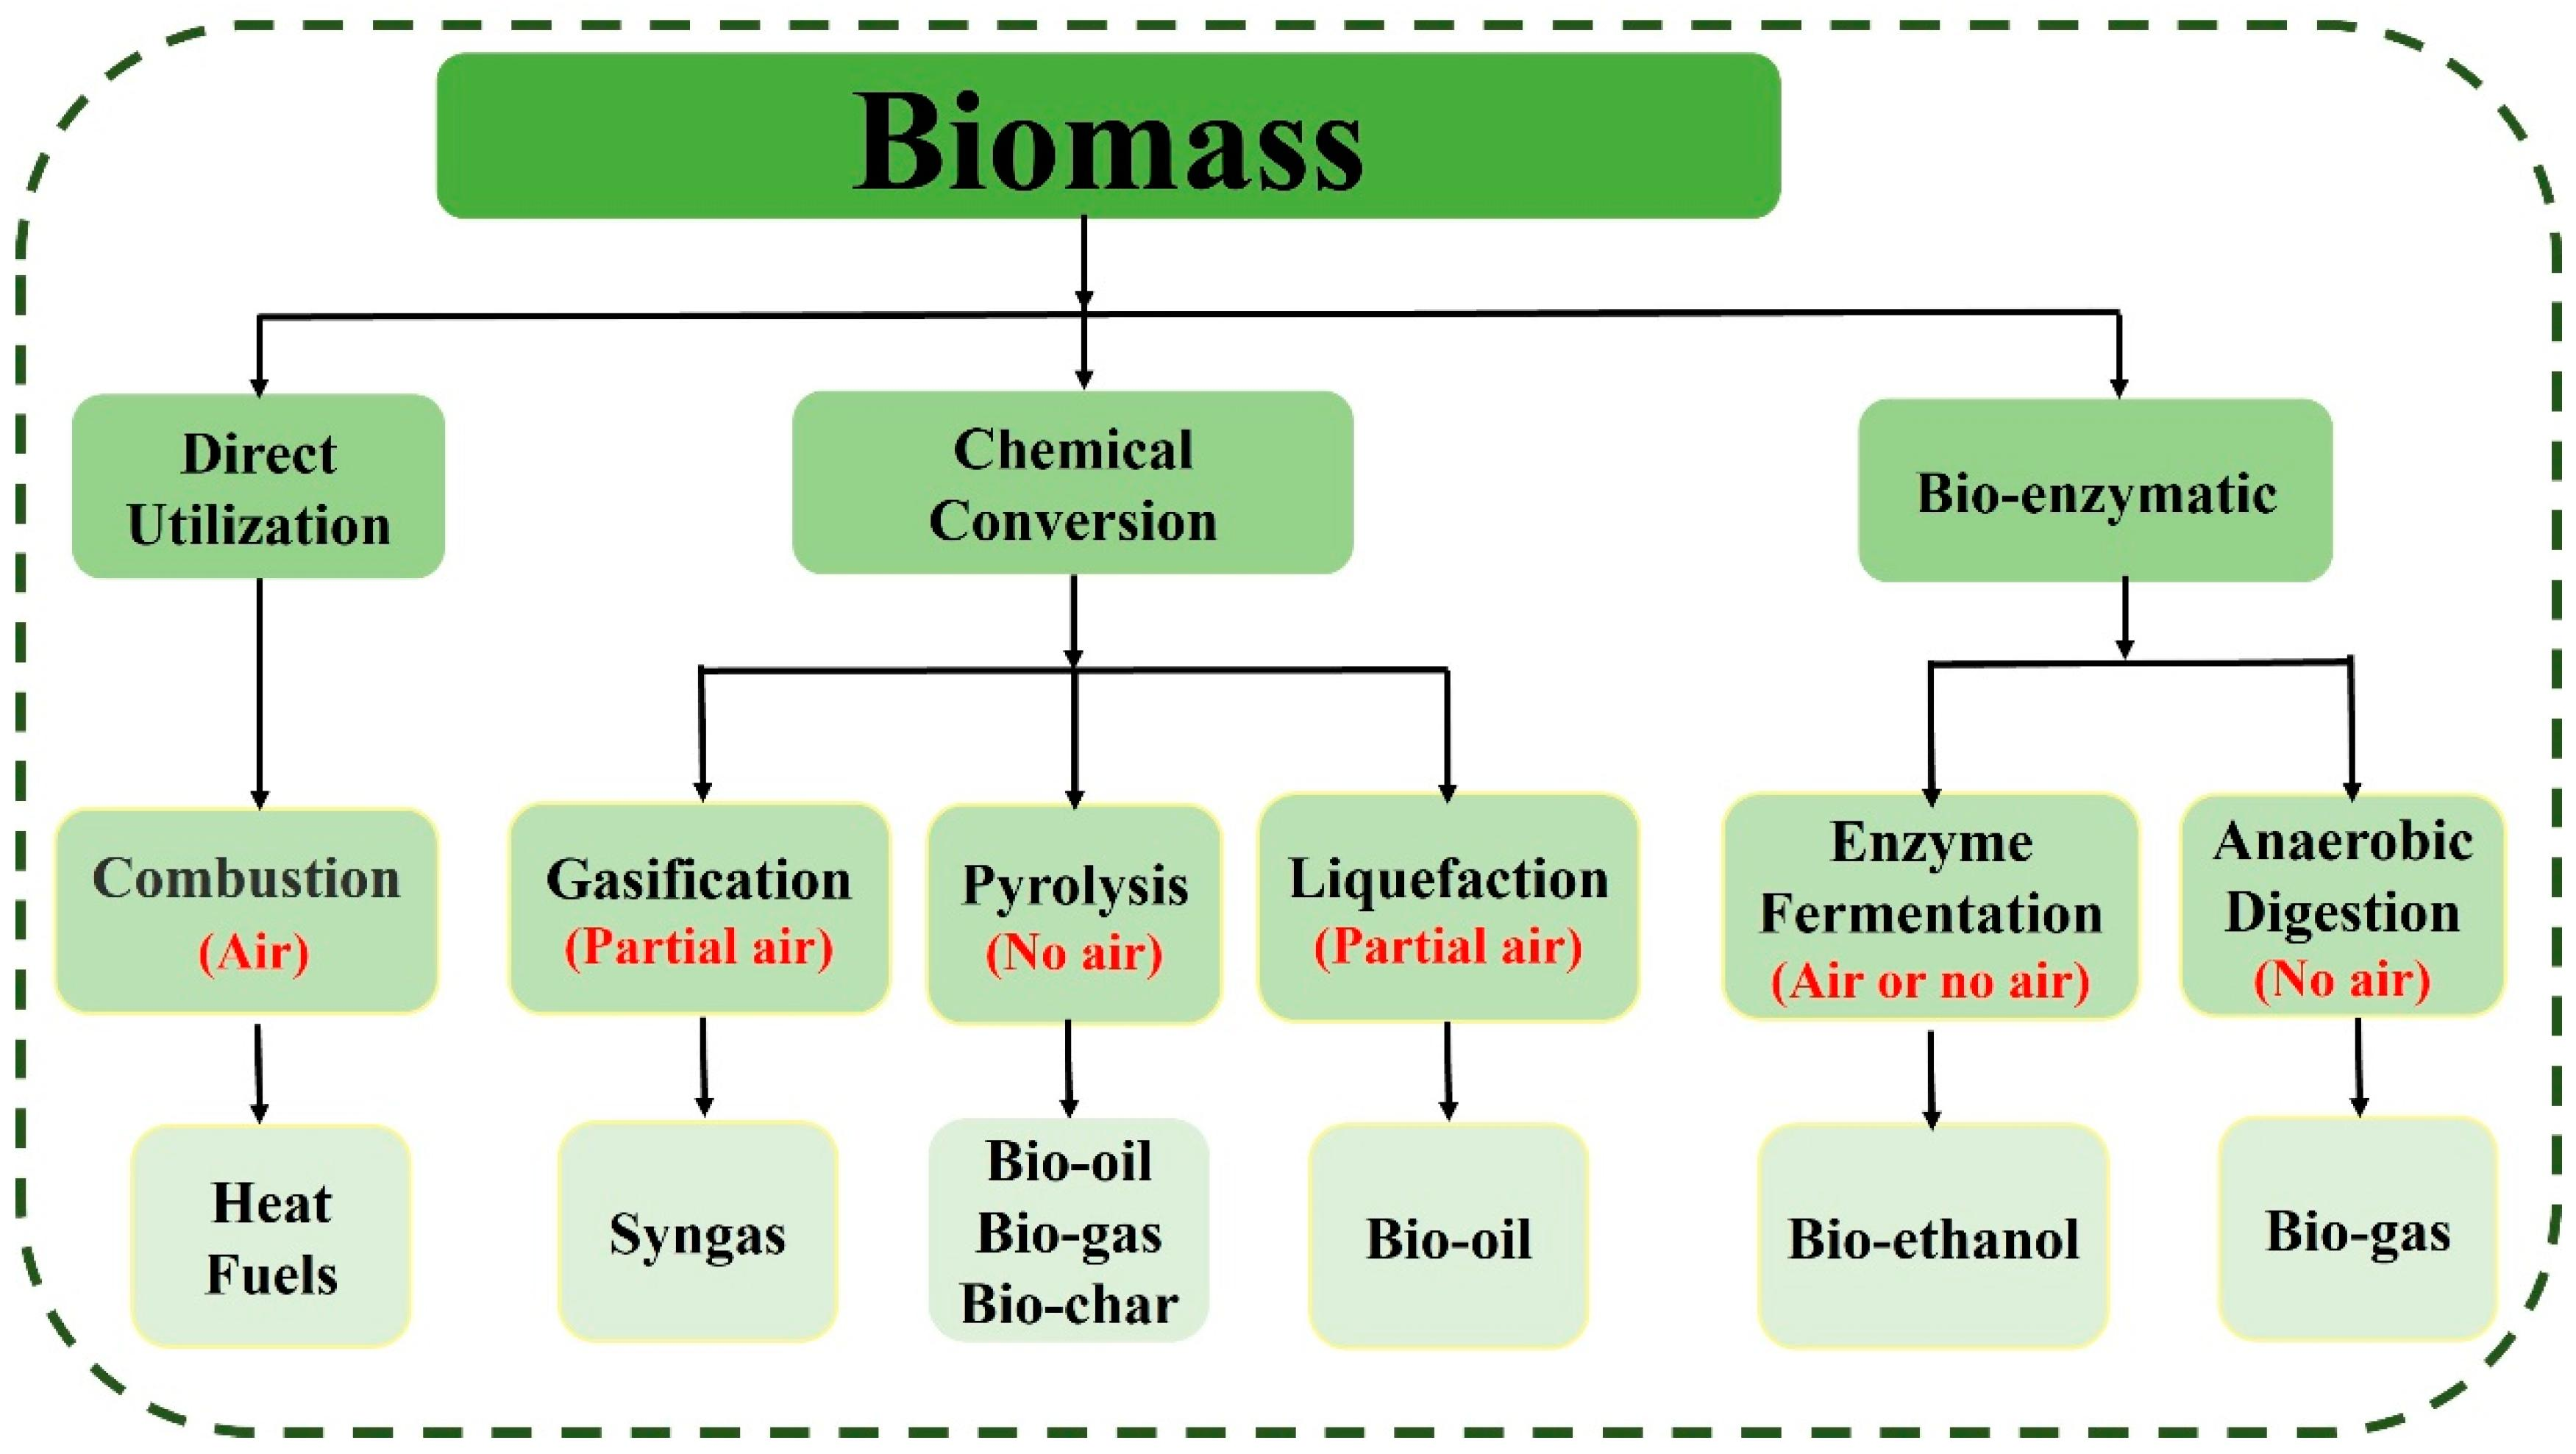
\includegraphics[width=0.9\textwidth]{Figuras/Sección B - Tecnologías de Conversión/Tecnologías de Conversión.jpg}
    \caption{Principales rutas de transformación de la biomasa en productos energéticos. Cada ruta depende de la naturaleza de la materia prima y del producto que se desea obtener}
\end{figure}

\section{Combustión directa}
\label{sec:combustion}

La combustión directa es la ruta tecnológica dominante y representa más del 90~\% de la contribución global de la bioenergía \cite{vanloo2007handbook}. Consiste en la oxidación completa de la biomasa con exceso de aire para liberar energía térmica, la cual se transfiere en una caldera para generar vapor destinado a procesos industriales o a la expansión en una turbina.

\subsection{Mecanismo y control de emisiones}
Dentro del hogar de la caldera, cada partícula de biomasa atraviesa cuatro etapas que ocurren de forma simultánea en distintas zonas:
\begin{enumerate}[leftmargin=1.5em]
\item \textbf{Calentamiento y secado} (hasta $\sim$100--150~\textdegree C): evaporación endotérmica de la humedad.
\item \textbf{Devolatilización} ($\sim$200--500~\textdegree C): liberación de materia volátil ($\mathrm{CO}$, $\mathrm{H_2}$, $\mathrm{CH_4}$, hidrocarburos y alquitranes), equivalente al 70--85~\% de la masa seca.
\item \textbf{Combustión de los volátiles} en fase gaseosa: forma la llama y libera la mayor fracción del calor.
\item \textbf{Combustión del carbonizado} (\textit{char}) en la superficie de la partícula, etapa más lenta que deja como residuo la ceniza.
\end{enumerate}

De forma global, la reacción de oxidación completa con aire puede representarse como:
\begin{equation}
\mathrm{CH}_x\mathrm{O}_y + a\left(\mathrm{O_2} + 3{,}76\,\mathrm{N_2}\right) \longrightarrow \mathrm{CO_2} + \mathrm{H_2O} + \mathrm{N_2} + \text{calor}
\end{equation}
Una combustión eficiente exige cumplir las denominadas «tres T»: \textit{temperatura} suficiente, \textit{tiempo de residencia} adecuado y \textit{turbulencia} para mezclar aire y gases. El aire se suministra escalonado en aire primario (bajo la parrilla o el lecho) y aire secundario (sobre el lecho, para quemar los volátiles), con excesos de aire típicos de 20--60~\%. Los principales contaminantes y sus sistemas de control se resumen en la Tabla~\ref{tab:emisiones_combustion}.

\begin{figure}[H]
    \centering
    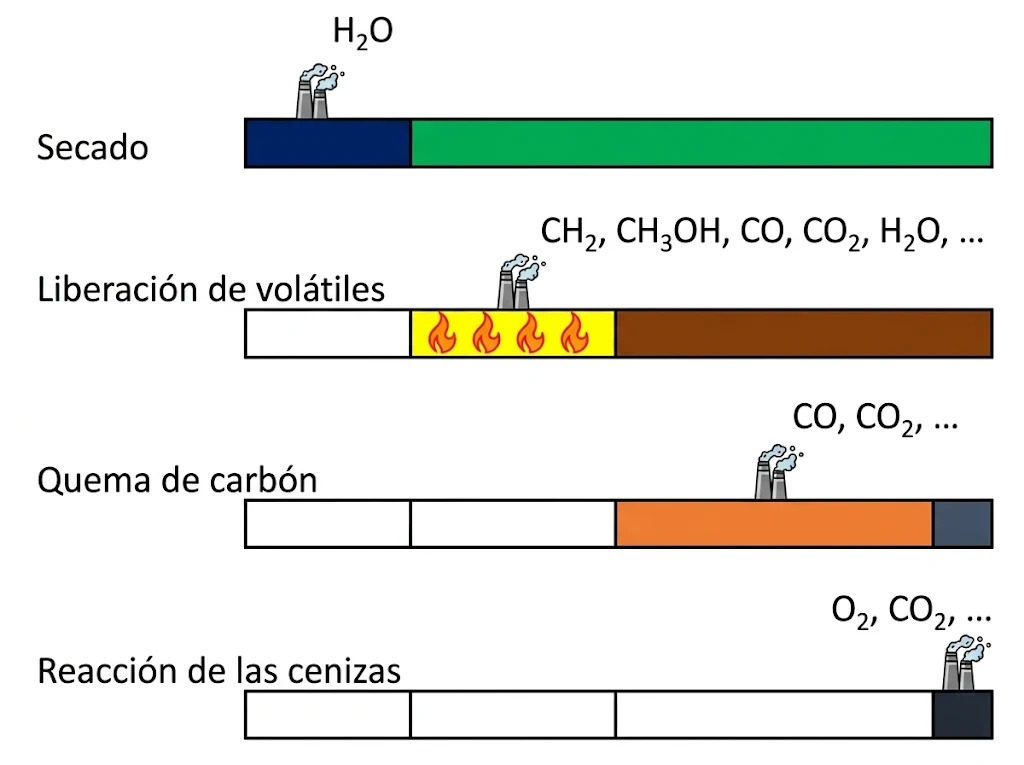
\includegraphics[width=0.9\textwidth]{Figuras/Sección B - Tecnologías de Conversión/Etapas de combustión de una partícula de biomasa.jpg}
    \caption{Etapas de secado, liberación de volátiles, combustión del carbonizado y formación de cenizas. Es la imagen más directamente relacionada con la explicación de tu mecanismo de combustión}
\end{figure}

\begin{table}[htbp]
\centering
\caption{Principales emisiones de la combustión de biomasa y tecnologías de control.}
\label{tab:emisiones_combustion}
\begin{tabularx}{\textwidth}{@{}l X X@{}}
\toprule
\textbf{Contaminante} & \textbf{Origen} & \textbf{Medidas de control} \\
\midrule
Material particulado & Cenizas volantes y aerosoles de sales alcalinas & Ciclones (partículas gruesas), filtros de mangas o precipitadores electrostáticos (partículas finas). \\
$\mathrm{CO}$ e hidrocarburos & Combustión incompleta por falta de aire, mala mezcla o baja temperatura & Aire secundario bien distribuido, control de exceso de aire (sonda $\mathrm{O_2}$) y tiempo de residencia. \\
$\mathrm{NO}_x$ & Principalmente nitrógeno del propio combustible ($\mathrm{NO}_x$ combustible) & Combustión por etapas, recirculación de gases, reducción selectiva no catalítica (SNCR con amoníaco o urea) o SCR. \\
$\mathrm{SO_2}$ y $\mathrm{HCl}$ & Azufre y cloro del combustible (bajos en madera, mayores en pajas) & Adición de caliza en el lecho o inyección de sorbentes secos. \\
\bottomrule
\end{tabularx}
\end{table}

\subsection{Equipos de combustión}
Las calderas industriales de biomasa se clasifican según la tecnología de hogar empleada (Tabla~\ref{tab:tecnologias_combustion}). Los lechos fluidizados circulantes (CFB) permiten unidades individuales mucho mayores que los burbujeantes (BFB), del orden de $300~\mathrm{MW_e}$ frente a $\sim 100~\mathrm{MW_e}$, con mayor flexibilidad de combustible \cite{flynn2005alholmens, irena2015heatpower}.

\begin{table}[htbp]
\centering
\caption{Tecnologías de combustión directa de biomasa \cite{irena2015heatpower, vanloo2007handbook}.}
\label{tab:tecnologias_combustion}
\begin{tabularx}{\textwidth}{@{}l l X X@{}}
\toprule
\textbf{Tecnología} & \textbf{Escala típica} & \textbf{Ventajas} & \textbf{Limitaciones} \\
\midrule
Parrilla fija & Pequeña & Simple y de bajo costo de inversión. & Exige combustible homogéneo; control limitado. \\
Parrilla móvil, vibratoria o inclinada & Pequeña a mediana & Madura para residuos de madera y bagazo; tolera combustibles húmedos. & Eficiencia y flexibilidad térmica intermedias. \\
Lecho fluidizado burbujeante (BFB) & Mediana & Excelente transferencia térmica; baja temperatura (800--900~\textdegree C) y menor $\mathrm{NO}_x$; admite combustibles heterogéneos. & Riesgo de aglomeración del lecho de arena con cenizas alcalinas. \\
Lecho fluidizado circulante (CFB) & Grande & Máxima flexibilidad de combustible y alta eficiencia en unidades de cientos de $\mathrm{MW_e}$. & Mayor costo de capital, consumo auxiliar y erosión interna. \\
Combustión pulverizada & Muy grande & Aprovecha calderas de carbón existentes; base de la co-combustión. & Requiere biomasa finamente molida o pellets. \\
\bottomrule
\end{tabularx}
\end{table}

\subsection{La caldera, balance global y ciclos de potencia}
La caldera integra el hogar, paredes de agua, sobrecalentador, economizador y precalentador de aire. Su eficiencia térmica sobre el PCI se sitúa entre 80 y 90~\%:
\begin{equation}
\eta_{\mathrm{caldera}} = \frac{\dot{Q}_{\text{útil}}}{\dot{m}_{\mathrm{comb}} \cdot \mathrm{PCI}}
\end{equation}

\begin{figure}[H]
    \centering
    \begin{subfigure}[b]{0.48\textwidth}
        \centering
        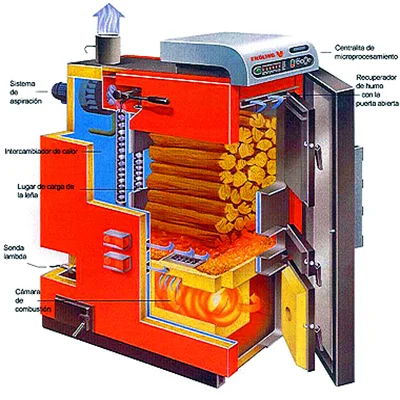
\includegraphics[width=\textwidth]{Figuras/Sección B - Tecnologías de Conversión/Combustión directa - CALDERA.jpg}
        \caption{Esquema de una caldera de combustión invertida para leña con sistema de tiro inducido, regulación por sonda lambda e intercambiador de calor vertical}
    \end{subfigure}
    \hfill
    \begin{subfigure}[b]{0.48\textwidth}
        \centering
        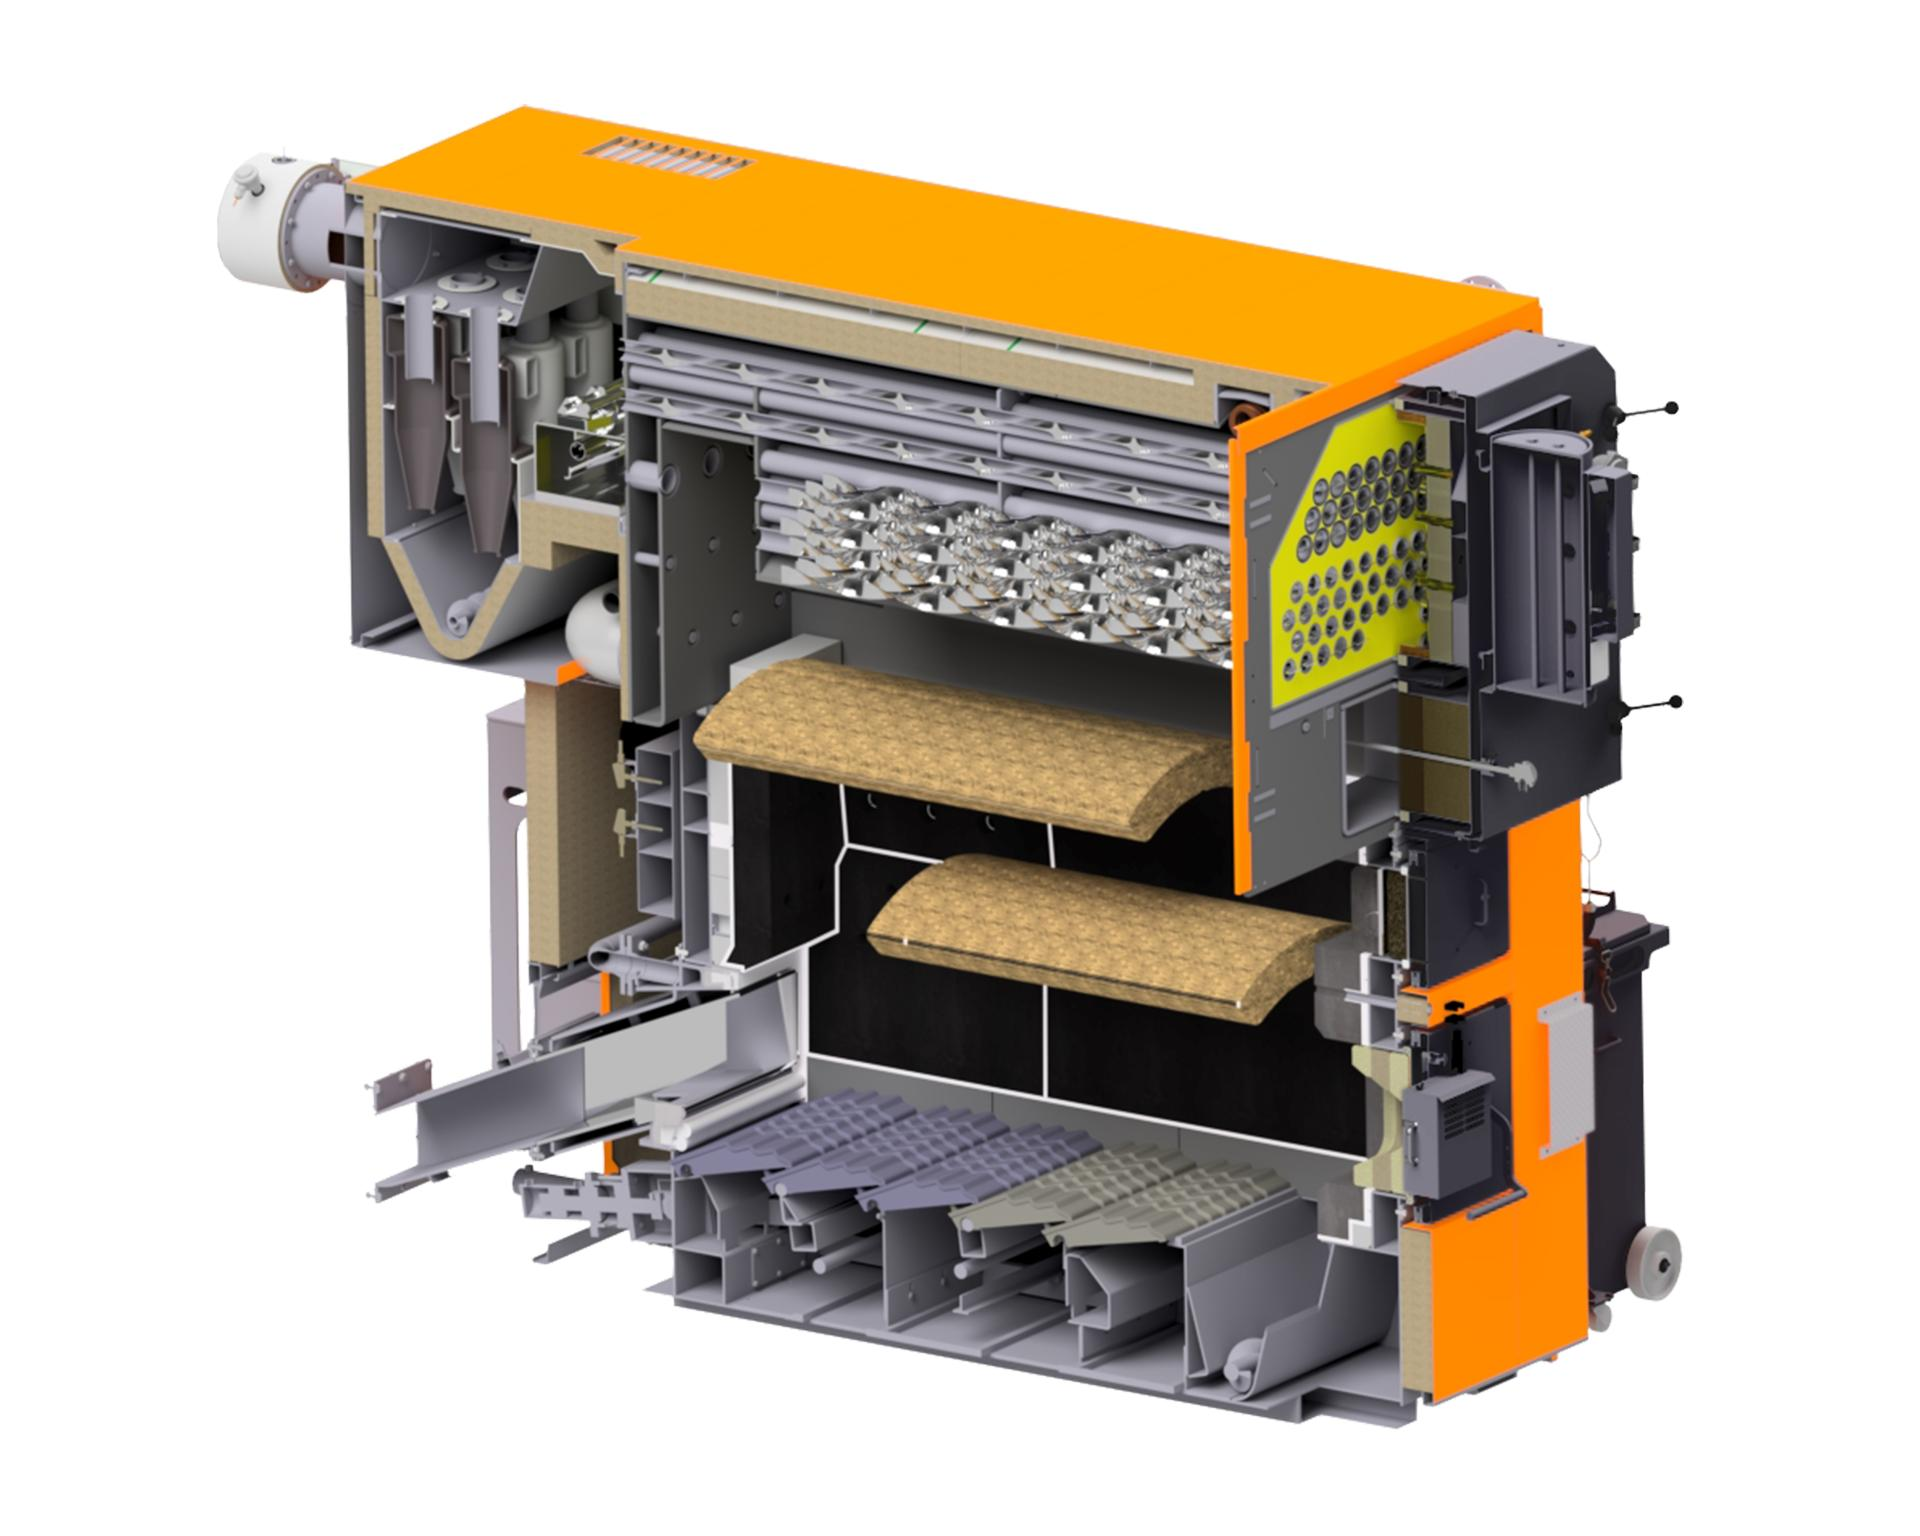
\includegraphics[width=\textwidth]{Figuras/Sección B - Tecnologías de Conversión/Combustión directa - Combustión en parrilla.jpg}
        \caption{Caldera de biomasa de parrilla escalonada móvil con bóvedas refractarias, intercambiador pirotubular horizontal y separador multiciclónico integrado}
    \end{subfigure}

    \caption{Tecnologías de calderas empleadas en la combustión directa de biomasa sólida}
    \label{fig:grupo_tres}
\end{figure}

Las principales pérdidas corresponden a los gases secos de chimenea (la mayor pérdida, creciente con el exceso de aire y temperatura de salida), la evaporación de la humedad del combustible, los inquemados (carbono en cenizas y $\mathrm{CO}$), y la radiación, convección y purgas. En parámetros de vapor, las plantas pequeñas operan a 20--60~bar y 400--450~\textdegree C, mientras que las grandes alcanzan 100--165~bar y 500--540~\textdegree C (límite impuesto por la corrosión por cenizas).

Como balance energético orientativo para una central dedicada mediana, de cada 100 unidades de energía del combustible (sobre PCI), entre 85 y 90 se transfieren al vapor; unas 55--60 se rechazan en el condensador; cerca de 30 salen como trabajo en el eje de la turbina; y tras descontar pérdidas de generador y consumos auxiliares (ventiladores, bombas y manejo de combustible, que representan 8--10~\% de la generación bruta), resultan alrededor de 25--28 unidades de electricidad neta.

Los ciclos termodinámicos aplicados son:
\begin{itemize}[leftmargin=1.5em]
\item \textbf{Ciclo Rankine de vapor:} Alcanza eficiencias eléctricas netas de 20--25~\% en pequeña escala y 30--35~\% en gran escala. Puede operar en condensación pura (maximiza electricidad) o en cogeneración mediante turbinas de contrapresión o extracción. Por ejemplo, Alholmens Kraft genera unos $240~\mathrm{MW_e}$ en condensación pura, o $205~\mathrm{MW_e}$ más $100~\mathrm{MW_{th}}$ de vapor de proceso y $60~\mathrm{MW_{th}}$ de calefacción urbana \cite{alholmenskraft}.
\item \textbf{Ciclo Rankine Orgánico (ORC):} Sustituye el agua por un fluido orgánico de bajo punto de ebullición (siloxanos o hidrocarburos) calentado mediante aceite térmico. Se emplea entre 0,2 y $5~\mathrm{MW_e}$ con eficiencia eléctrica de 15--20~\%, destacando por su operación automatizada, buen desempeño a carga parcial y ausencia de planta de tratamiento de agua.
\item \textbf{Co-combustión y conversión total:} La co-combustión quema biomasa junto con carbón de forma directa (mezcla en molinos o quemadores), indirecta (gasificación previa) o paralela (caldera independiente). Es comercialmente viable hasta un 20~\% en base energética y técnicamente puede superar el 50~\%, alcanzando eficiencias eléctricas de 36--44~\% \cite{irena2013cofiring}. El paso siguiente es la conversión total de la central, como en el caso de Drax \cite{drax2025annual}.
\end{itemize}

\begin{figure}[H]
    \centering
    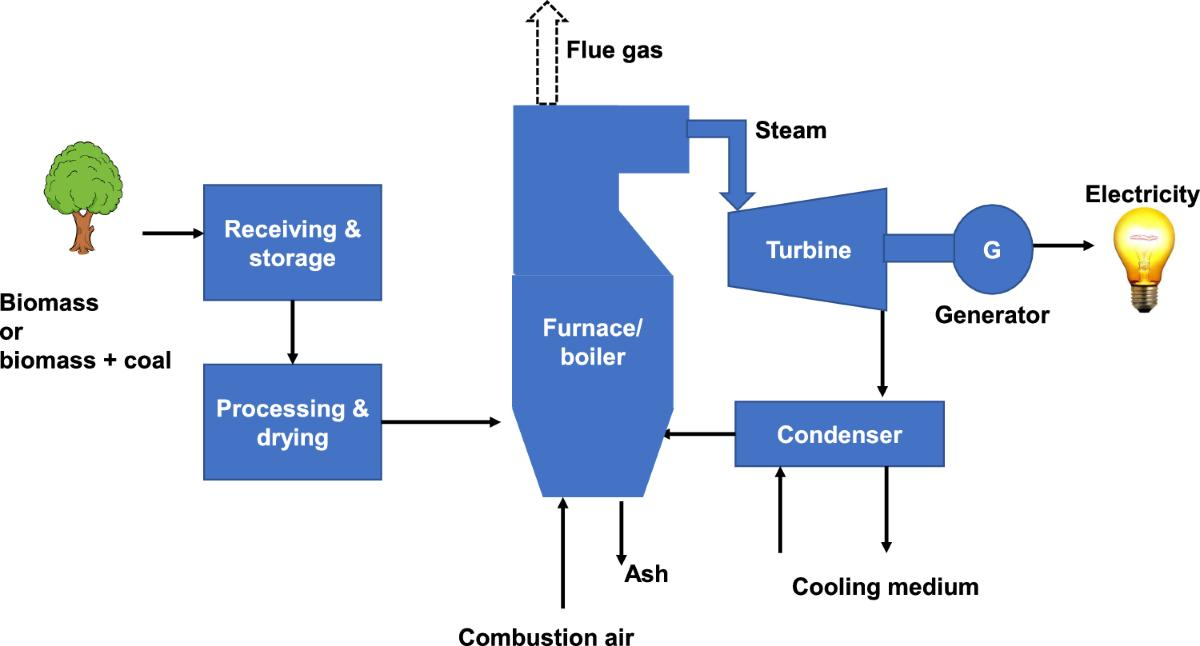
\includegraphics[width=0.9\textwidth]{Figuras/Sección B - Tecnologías de Conversión/Combustión directa - Generación de electricidad.jpg}
    \caption{Esquema de generación eléctrica mediante combustión de biomasa y ciclo Rankine}
\end{figure}

\section{Gasificación}
\label{sec:gasificacion}

La gasificación es la descomposición térmica de la biomasa en una atmósfera reductora de aire, oxígeno o vapor de agua en cantidad subestequiométrica ($\lambda \approx 0{,}2\text{--}0{,}4$) para producir un gas combustible denominado \textit{gas de síntesis} o \textit{syngas} \cite{ieabioenergy2025task33, idae2007gasificacion}. La oxidación parcial aporta el calor necesario para sostener las reacciones de reducción, mayoritariamente endotérmicas.

\subsection{Mecanismo y reacciones principales}
En un gasificador de lecho fijo se distinguen cuatro zonas sucesivas: secado (100--200~\textdegree C), pirólisis (200--600~\textdegree C), oxidación (900--1\,200~\textdegree C) y reducción (700--900~\textdegree C). Las reacciones químicas fundamentales se detallan en la Tabla~\ref{tab:reacciones_gasificacion}.

\begin{table}[htbp]
\centering
\caption{Reacciones principales de la gasificación (entalpías de referencia a 25~\textdegree C).}
\label{tab:reacciones_gasificacion}
\begin{tabular}{@{}llrl@{}}
\toprule
\textbf{Reacción} & \textbf{Ecuación} & \textbf{$\Delta H$ (kJ/mol)} & \textbf{Carácter térmico} \\
\midrule
Combustión completa & $\mathrm{C} + \mathrm{O_2} \longrightarrow \mathrm{CO_2}$ & $-394$ & Exotérmica (aporta calor) \\
Combustión parcial & $\mathrm{C} + \frac{1}{2}\,\mathrm{O_2} \longrightarrow \mathrm{CO}$ & $-111$ & Exotérmica \\
Boudouard & $\mathrm{C} + \mathrm{CO_2} \rightleftharpoons 2\,\mathrm{CO}$ & $+172$ & Endotérmica \\
Agua-gas & $\mathrm{C} + \mathrm{H_2O} \rightleftharpoons \mathrm{CO} + \mathrm{H_2}$ & $+131$ & Endotérmica \\
Desplazamiento (\textit{shift}) & $\mathrm{CO} + \mathrm{H_2O} \rightleftharpoons \mathrm{CO_2} + \mathrm{H_2}$ & $-41$ & Ligeramente exotérmica \\
Metanación & $\mathrm{C} + 2\,\mathrm{H_2} \rightleftharpoons \mathrm{CH_4}$ & $-75$ & Exotérmica \\
\bottomrule
\end{tabular}
\end{table}

\subsection{Agente gasificante, calidad del gas y tipos de reactores}
El agente gasificante determina el poder calorífico del gas obtenido (Tabla~\ref{tab:agente_gasificante}). Con aire, la dilución con nitrógeno reduce el PCI a 4--6~MJ/Nm$^3$ (frente a $\sim 35~\text{MJ/Nm}^3$ del gas natural). El punto de operación habitual con aire se ubica en $\lambda \approx 0{,}25\text{--}0{,}35$: valores inferiores disminuyen la temperatura y aumentan los alquitranes, mientras que valores superiores queman parte del gas producido. La eficiencia de gas frío (\textit{Cold Gas Efficiency}) suele ubicarse entre 65 y 80~\%:
\begin{equation}
\eta_{\text{gas frío}} = \frac{\dot{m}_{\mathrm{gas}} \cdot \mathrm{PCI}_{\mathrm{gas}}}{\dot{m}_{\mathrm{comb}} \cdot \mathrm{PCI}_{\mathrm{comb}}}
\end{equation}

\begin{table}[htbp]
\centering
\caption{Calidad del syngas según el agente gasificante (valores orientativos).}
\label{tab:agente_gasificante}
\begin{tabularx}{\textwidth}{@{}l l X X@{}}
\toprule
\textbf{Agente} & \textbf{PCI del gas} & \textbf{Composición típica} & \textbf{Aplicación} \\
\midrule
Aire & 4--6~MJ/Nm$^3$ & $\mathrm{CO}$ 15--20~\%, $\mathrm{H_2}$ 10--20~\%, $\mathrm{CH_4}$ 1--5~\%, $\mathrm{CO_2}$ 10--15~\%, $\mathrm{N_2}$ 45--55~\% & Motores de combustión interna y calderas; opción más económica. \\
Oxígeno & 10--15~MJ/Nm$^3$ & Libre de $\mathrm{N_2}$; rico en $\mathrm{CO}$ y $\mathrm{H_2}$ & Turbinas de gas y síntesis de combustibles; requiere planta de $\mathrm{O_2}$. \\
Vapor (indirecta) & 12--15~MJ/Nm$^3$ & Libre de $\mathrm{N_2}$; alto contenido de $\mathrm{H_2}$ & Síntesis química y producción de hidrógeno. \\
\bottomrule
\end{tabularx}
\end{table}

Según la configuración hidrodinámica entre biomasa y agente gasificante se distinguen cuatro tipos de reactores (Tabla~\ref{tab:tipos_gasificadores}).

\begin{table}[htbp]
\centering
\small
\caption{Clasificación de reactores de gasificación de biomasa \cite{fao1986woodgas, idae2007gasificacion}.}
\label{tab:tipos_gasificadores}
\begin{tabularx}{\textwidth}{@{}p{2.5cm} p{2.3cm} p{2.1cm} X X@{}}
\toprule
\textbf{Tipo} & \textbf{Flujo} & \textbf{Escala} & \textbf{Ventajas} & \textbf{Limitaciones} \\
\midrule
Lecho fijo \textit{updraft} & Contracorriente & Pequeña & Alta eficiencia térmica; tolera humedad. & Alto contenido de alquitranes; uso térmico directo. \\
Lecho fijo \textit{downdraft} & Co-corriente & Pequeña ($\le 1~\mathrm{MW_e}$) & Craquea los alquitranes; gas apto para motores. & Exige combustible seco y granulometría uniforme. \\
Lecho fluidizado (BFB/CFB) & Arena fluidizada & Mediana a grande & Flexible y escalable. & Alquitranes y partículas intermedios. \\
Flujo arrastrado & Partícula fina ($>1\,200$~\textdegree C) & Muy grande & Gas prácticamente libre de alquitrán. & Requiere molienda intensiva; orientado a síntesis. \\
\bottomrule
\end{tabularx}
\end{table}

El principal obstáculo técnico de la gasificación son los \textbf{alquitranes}, hidrocarburos pesados que condensan al enfriarse y obstruyen filtros, válvulas y motores. Para su uso en motores de combustión interna, el gas debe enfriarse y limpiarse mediante ciclones, filtros, lavadores (\textit{scrubbers}) o craqueo catalítico hasta niveles inferiores a 50--100~mg/Nm$^3$ de alquitrán \cite{fao1986woodgas}. Acoplado a motores de gas (o motores diésel en modo dual), el conjunto alcanza eficiencias eléctricas de 20--30~\%, mientras que la gasificación integrada en ciclo combinado (BIGCC) proyecta 35--45~\%, aunque permanece en fase de demostración \cite{ieabioenergy2025task33}.

\begin{figure}[H]
    \centering
    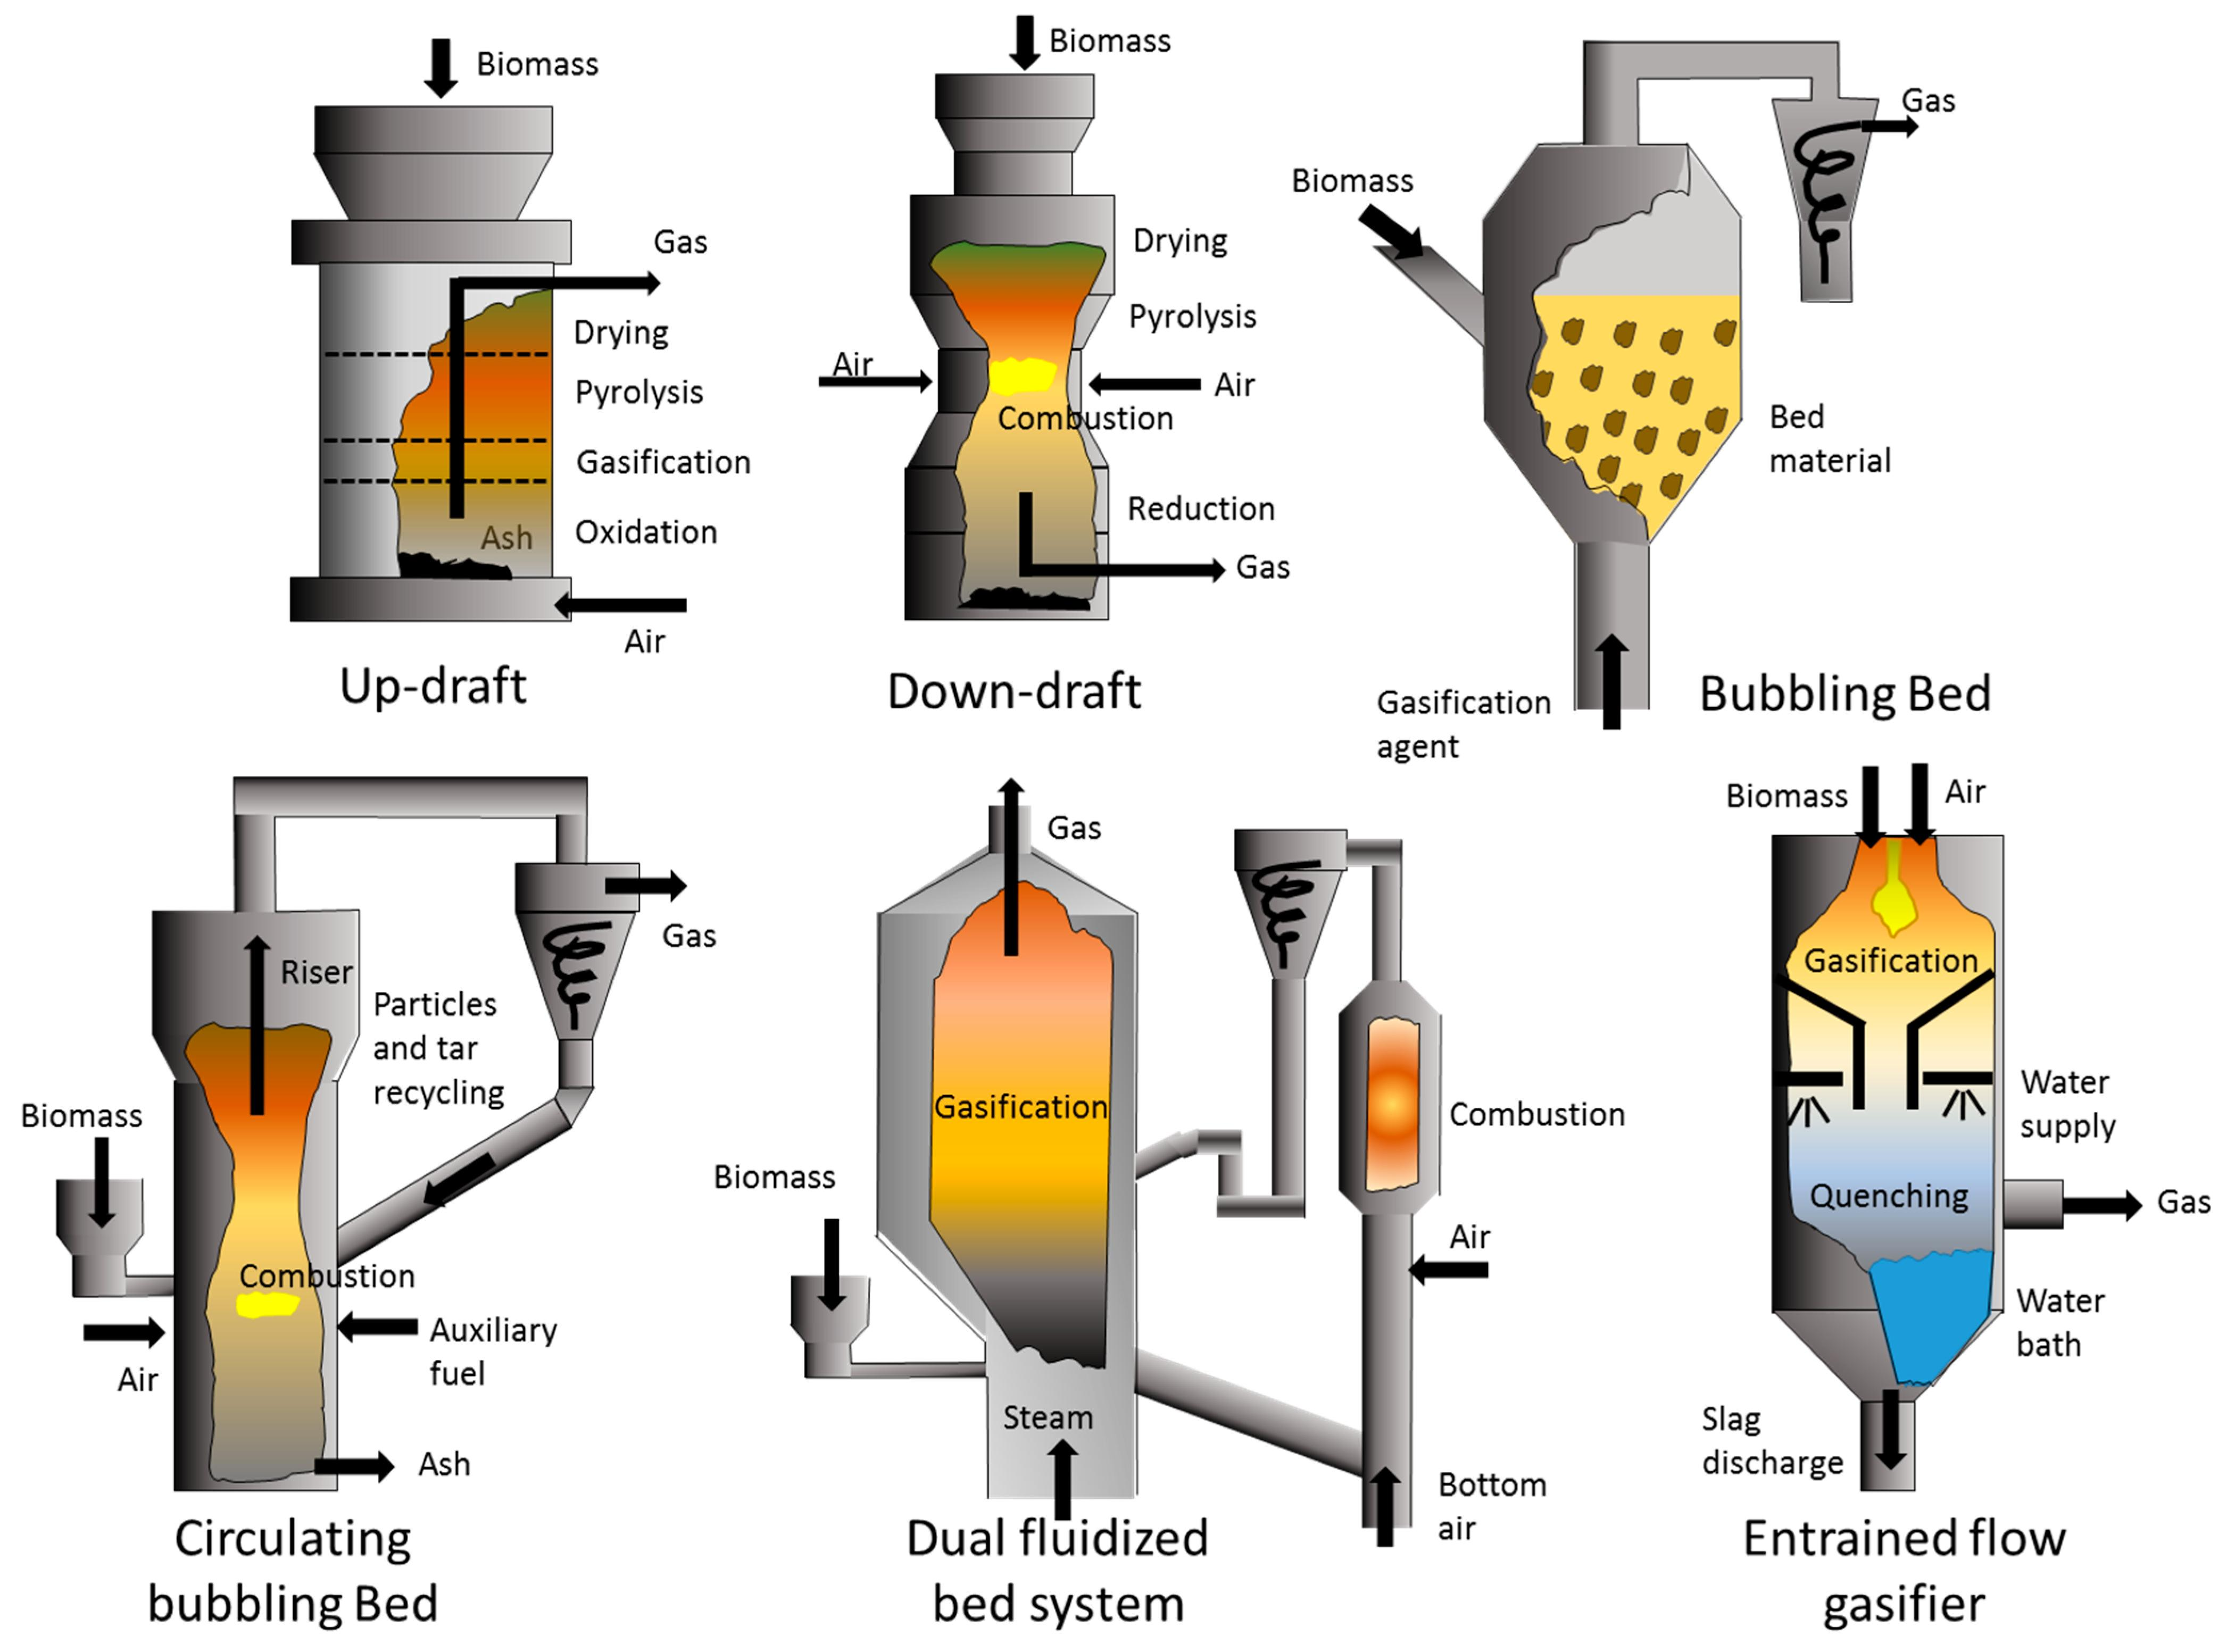
\includegraphics[width=0.8\textwidth]{Figuras/Sección B - Tecnologías de Conversión/Comparación de los tipos de gasificadores.jpg}
    \caption{Comparación esquemática de diferentes configuraciones de gasificadores, incluyendo lecho fijo ascendente (updraft), descendente (downdraft), lecho fluidizado y flujo arrastrado. Se muestran las direcciones de alimentación de biomasa, entrada del agente gasificante y salida del gas producido}
\end{figure}

\begin{figure}[H]
    \centering
    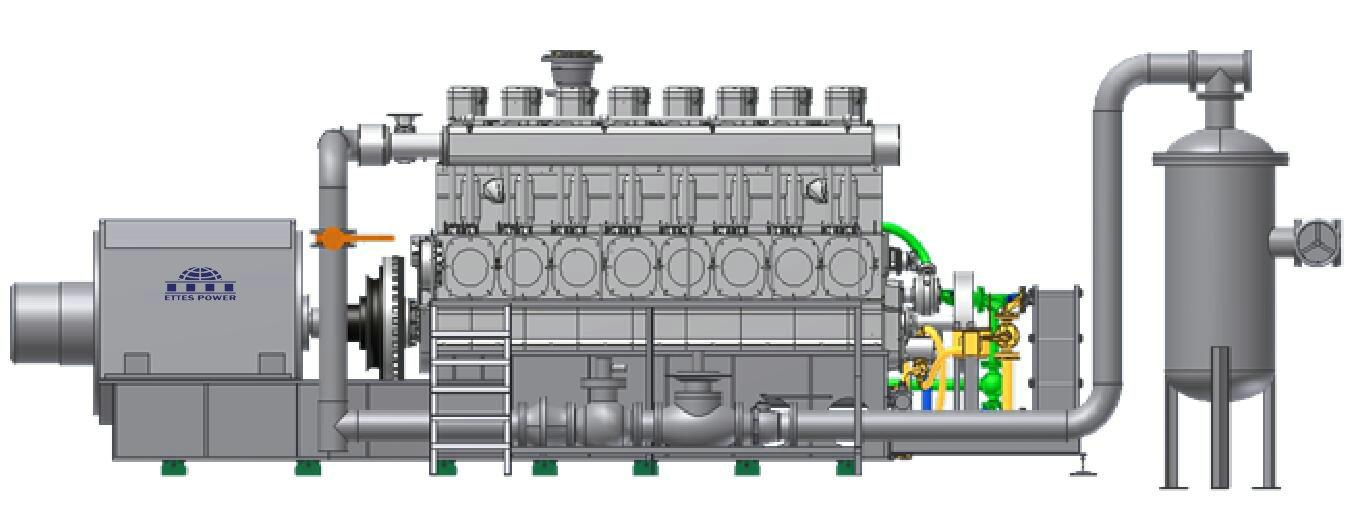
\includegraphics[width=0.8\textwidth]{Figuras/Sección B - Tecnologías de Conversión/Aprovechamiento energético del syngas.jpg}
    \caption{Conjunto motor-generador diseñado para utilizar gas de síntesis como combustible. La combustión del gas dentro del motor produce energía mecánica que acciona un generador eléctrico, permitiendo transformar la energía química del syngas en electricidad}
\end{figure}

\section{Pirólisis}
\label{sec:pirolisis}

La pirólisis es la descomposición térmica de la biomasa en ausencia total de oxígeno ($\lambda = 0$), típicamente entre 300 y 700~\textdegree C \cite{bridgwater2012pyrolysis}. A partir de un balance de masa, la biomasa alimentada se distribuye en tres fracciones: sólida (\textit{biochar}), líquida (\textit{bio-oil} o bioaceite) y gaseosa ($\mathrm{CO}$, $\mathrm{CO_2}$, $\mathrm{H_2}$, $\mathrm{CH_4}$):
\begin{equation}
m_{\mathrm{biomasa}} = m_{\text{bio-oil}} + m_{\mathrm{biochar}} + m_{\mathrm{gas}}
\end{equation}
La proporción relativa depende de la temperatura, velocidad de calentamiento y tiempo de residencia de los vapores (Tabla~\ref{tab:pirolisis_modos}). La pirólisis rápida emplea reactores de lecho fluidizado burbujeante, cono rotatorio o tornillo sinfín con condensación brusca de vapores.

\begin{figure}[H]
    \centering
    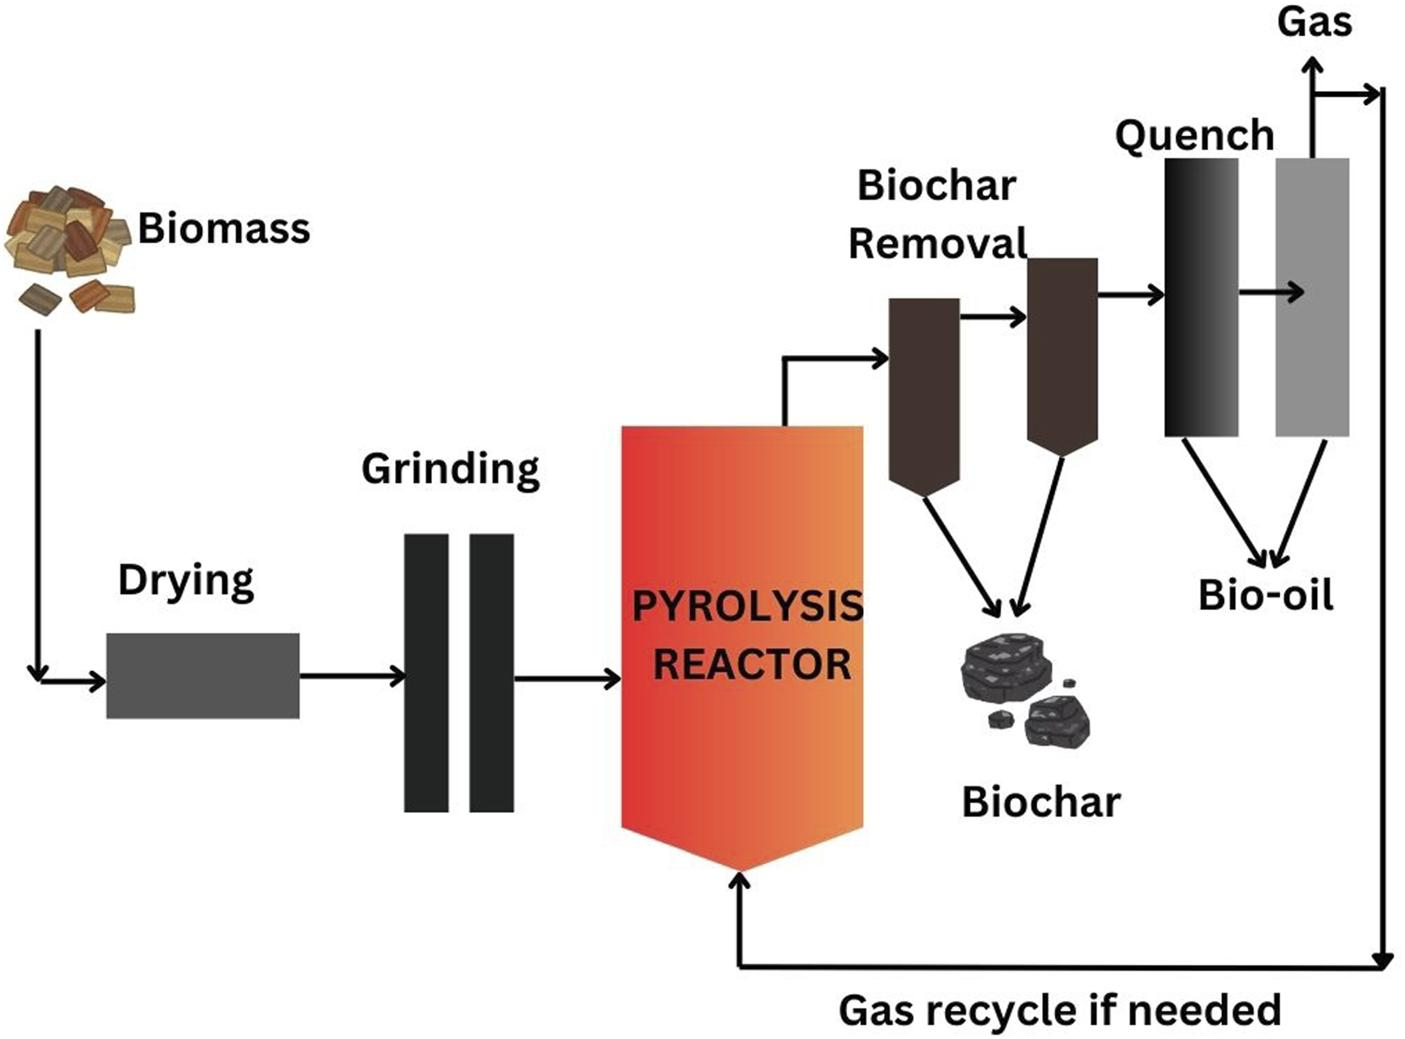
\includegraphics[width=0.8\textwidth]{Figuras/Sección B - Tecnologías de Conversión/Conversón termoquímica - Diagrama de pirólisis.jpg}
    \caption{Diagrama de flujo del proceso de pirólisis de biomasa, incluyendo las etapas de pretratamiento, reacción y separación de productos (biocarbón, bioaceite y gas).}
\end{figure}

\begin{table}[htbp]
\centering
\caption{Distribución típica de productos en pirólisis (porcentaje en masa de biomasa seca) \cite{bridgwater2012pyrolysis}.}
\label{tab:pirolisis_modos}
\begin{tabularx}{\textwidth}{@{}l X ccc@{}}
\toprule
\textbf{Modo} & \textbf{Condiciones típicas} & \textbf{Líquido} & \textbf{Sólido} & \textbf{Gas} \\
\midrule
Lenta (carbonización) & 300--500~\textdegree C; horas a días & $\approx 30~\%$ & $\approx 35~\%$ & $\approx 35~\%$ \\
Intermedia & $\approx 500$~\textdegree C; residencia de vapores 10--30~s & $\approx 50~\%$ & $\approx 25~\%$ & $\approx 25~\%$ \\
Rápida & $\approx 500$~\textdegree C; vapores $\sim 1$~s; enfriamiento brusco & $\approx 75~\%$ & $\approx 12~\%$ & $\approx 13~\%$ \\
Gasificación (ref.) & 750--900~\textdegree C ($\lambda \approx 0{,}2\text{--}0{,}4$) & $\approx 5~\%$ & $\approx 10~\%$ & $\approx 85~\%$ \\
\bottomrule
\end{tabularx}
\end{table}

El valor estratégico de la pirólisis rápida reside en transformar una biomasa voluminosa en un líquido denso y transportable (\textit{bio-oil}), resolviendo parte del problema logístico. Sin embargo, el bioaceite presenta propiedades exigentes frente al fuel oil pesado (Tabla~\ref{tab:biooil}): contiene 15--30~\% de agua, alto oxígeno (35--40~\%), pH ácido (2--3, corrosivo) e inestabilidad por envejecimiento \cite{elliott2017roundrobin}. Por ello, raramente se usa para generación eléctrica directa, empleándose en calderas adaptadas o plantas integradas de cogeneración como Joensuu (Finlandia) y Empyro (Países Bajos) \cite{ieabioenergy_task34}. El \textit{biochar} se destina a enmienda de suelos, secuestro de carbono o combustible sólido.

\begin{table}[htbp]
\centering
\caption{Propiedades típicas del bioaceite de pirólisis rápida frente al fuel oil pesado.}
\label{tab:biooil}
\begin{tabular}{@{}lcc@{}}
\toprule
\textbf{Propiedad} & \textbf{Bio-oil (típico)} & \textbf{Fuel oil pesado (ref.)} \\
\midrule
Poder calorífico inferior & 16--19~MJ/kg & $\approx 40$~MJ/kg \\
Contenido de agua & 15--30~\% & $< 1~\%$ \\
Acidez & pH 2--3 (corrosivo) & Neutro \\
Contenido de oxígeno & 35--40~\% & $\approx 1~\%$ \\
Estabilidad & Envejece (aumenta viscosidad) & Estable \\
Miscibilidad con hidrocarburos & No miscible & --- \\
\bottomrule
\end{tabular}
\end{table}

\section{Digestión anaeróbica}
\label{sec:digestion}

La digestión anaeróbica es un proceso bioquímico en el que un consorcio de microorganismos descompone la materia orgánica en ausencia de oxígeno para producir \textbf{biogás} y un residuo estabilizado rico en nutrientes denominado \textbf{digestato} \cite{alseadi2008biogas, idae2007digestores}. Constituye la ruta idónea para sustratos muy húmedos (estiércoles, lodos de depuradoras, efluentes agroindustriales y fracción orgánica de residuos urbanos), inviables en rutas térmicas \cite{ieabioenergy2024task37}.

\begin{figure}[H]
    \centering
    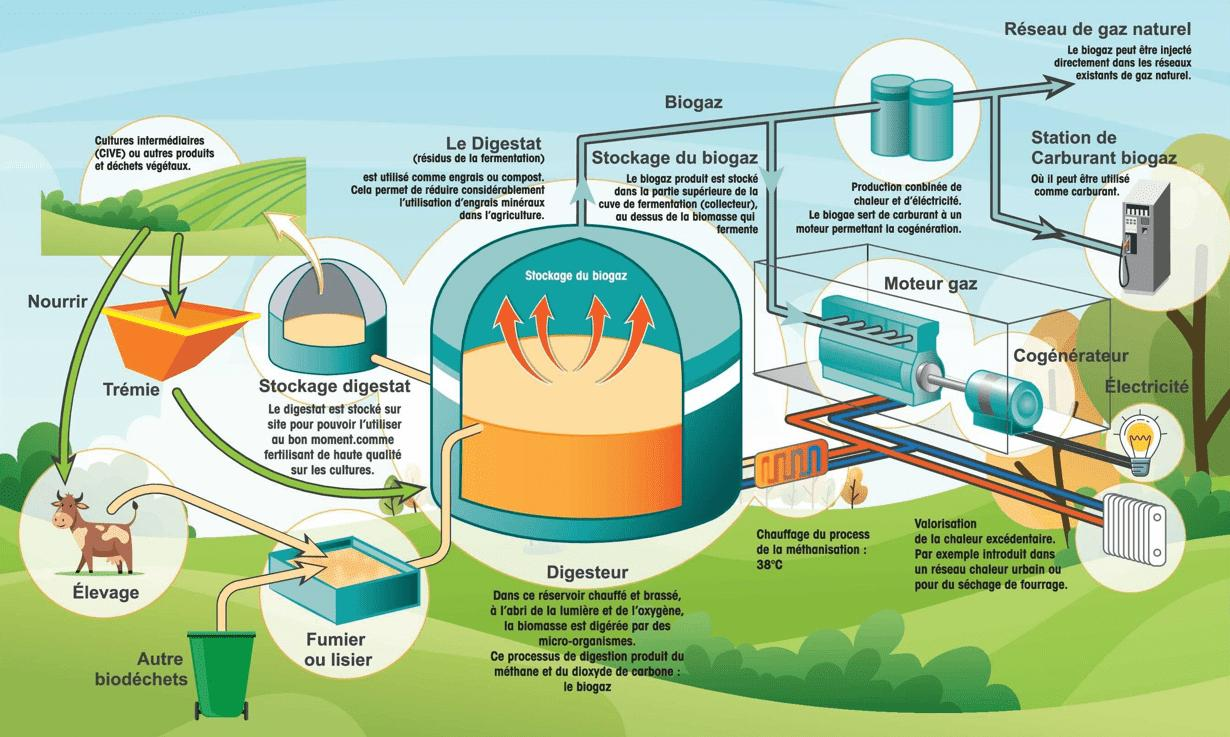
\includegraphics[width=0.8\textwidth]{Figuras/Sección B - Tecnologías de Conversión/Esquema general del proceso de digestión anaeróbica.jpg}
    \caption{Representación de las principales etapas de una planta de digestión anaeróbica, desde la alimentación de residuos orgánicos hasta su descomposición en el digestor}
\end{figure}

\subsection{Etapas y parámetros de operación}
El proceso biológico transcurre en cuatro etapas secuenciales:
\begin{enumerate}[leftmargin=1.5em]
\item \textbf{Hidrólisis:} enzimas extracelulares rompen carbohidratos, proteínas y lípidos en monómeros solubles (etapa limitante en sustratos fibrosos).
\item \textbf{Acidogénesis:} bacterias fermentativas transforman dichos compuestos en ácidos grasos volátiles (AGV), alcoholes, $\mathrm{H_2}$ y $\mathrm{CO_2}$.
\item \textbf{Acetogénesis:} los AGV se convierten en ácido acético, $\mathrm{H_2}$ y $\mathrm{CO_2}$.
\item \textbf{Metanogénesis:} arqueas metanogénicas producen metano por vía acetoclástica ($\sim 70~\%$) e hidrogenotrófica:
\begin{equation}
\mathrm{CH_3COOH} \longrightarrow \mathrm{CH_4} + \mathrm{CO_2}, \qquad \mathrm{CO_2} + 4\,\mathrm{H_2} \longrightarrow \mathrm{CH_4} + 2\,\mathrm{H_2O}
\end{equation}
\end{enumerate}

Los parámetros críticos de control se muestran en la Tabla~\ref{tab:parametros_digestion}. El volumen útil del digestor se dimensiona a partir del caudal diario de sustrato ($Q$) y el tiempo de retención hidráulica ($\mathrm{TRH}$) como $V = Q \cdot \mathrm{TRH}$, operando habitualmente en mezcla completa mesófila con cargas orgánicas volumétricas de 2--5~kg~SV/(m$^3\cdot$día) para evitar la acidificación del reactor.

\begin{table}[htbp]
\centering
\caption{Parámetros de operación de la digestión anaeróbica \cite{alseadi2008biogas, idae2007digestores}.}
\label{tab:parametros_digestion}
\begin{tabularx}{\textwidth}{@{}l l X@{}}
\toprule
\textbf{Parámetro} & \textbf{Valor típico} & \textbf{Importancia operativa} \\
\midrule
Temperatura & Mesófila 30--40~\textdegree C ($\sim 37$~\textdegree C); termófila 50--60~\textdegree C & La termófila acelera la cinética, pero es más inestable y consume mayor calor. \\
pH & 6,5--7,5 & Las arqueas metanogénicas son muy sensibles a la acidificación. \\
TRH & 15--30 días (régimen mesófilo) & Define el volumen útil del digestor. \\
Relación C/N & 20--30 & Un déficit de carbono acumula amoníaco e inhibe el proceso. \\
Inhibidores & Amoníaco, $\mathrm{H_2S}$, exceso de AGV, antibióticos & Pueden reducir o detener la producción de metano. \\
\bottomrule
\end{tabularx}
\end{table}

\subsection{Rendimientos, equipos y tratamiento del biogás}
El biogás contiene 50--70~\% de $\mathrm{CH_4}$ y 30--50~\% de $\mathrm{CO_2}$, más vapor de agua y trazas de $\mathrm{H_2S}$, con un PCI de 20--25~MJ/Nm$^3$. Con 60~\% de metano ($21{,}5~\text{MJ/Nm}^3$), $1~\text{Nm}^3$ equivale a $\sim 6~\text{kWh}$ térmicos, generando $\approx 2\text{--}2{,}3~\text{kWh}$ eléctricos en un motogenerador Otto de 35--40~\% de eficiencia. Los rendimientos varían notablemente según el sustrato (Tabla~\ref{tab:rendimientos_biogas}).

\begin{table}[htbp]
\centering
\caption{Rendimientos orientativos de biogás por tipo de sustrato.}
\label{tab:rendimientos_biogas}
\begin{tabular}{@{}lc@{}}
\toprule
\textbf{Sustrato} & \textbf{Biogás por tonelada fresca (Nm$^3$/t)} \\
\midrule
Estiércol vacuno o porcino & 15--35 \\
Gallinaza & 40--80 \\
Residuos de alimentos / fracción orgánica de RSU & 100--150 \\
Ensilaje de maíz & 170--220 \\
\bottomrule
\end{tabular}
\end{table}

Para ilustrar la escala, un motogenerador de $1~\mathrm{MW_e}$ al 38~\% de eficiencia requiere $1 / 0{,}38 \approx 2{,}63~\mathrm{MW_{th}}$ de biogás ($\approx 440~\text{Nm}^3/\text{h}$ o $10\,600~\text{Nm}^3/\text{día}$ a $21{,}5~\text{MJ/Nm}^3$). Con estiércol a $25~\text{Nm}^3/\text{t}$, ello exige $\approx 420~\text{t/día}$ y un digestor de $V \approx 420 \times 25 \approx 10\,500~\text{m}^3$ ($\mathrm{TRH}=25$~días), razón por la cual estas plantas suelen ser de pequeña escala o recurren a co-digestión. Entre los reactores empleados destacan las lagunas cubiertas (climas cálidos y efluentes agroindustriales), reactores de mezcla completa (CSTR), flujo pistón, reactores UASB (aguas industriales de alta carga) y pozos de captación en rellenos sanitarios.

\begin{figure}[H]
    \centering
    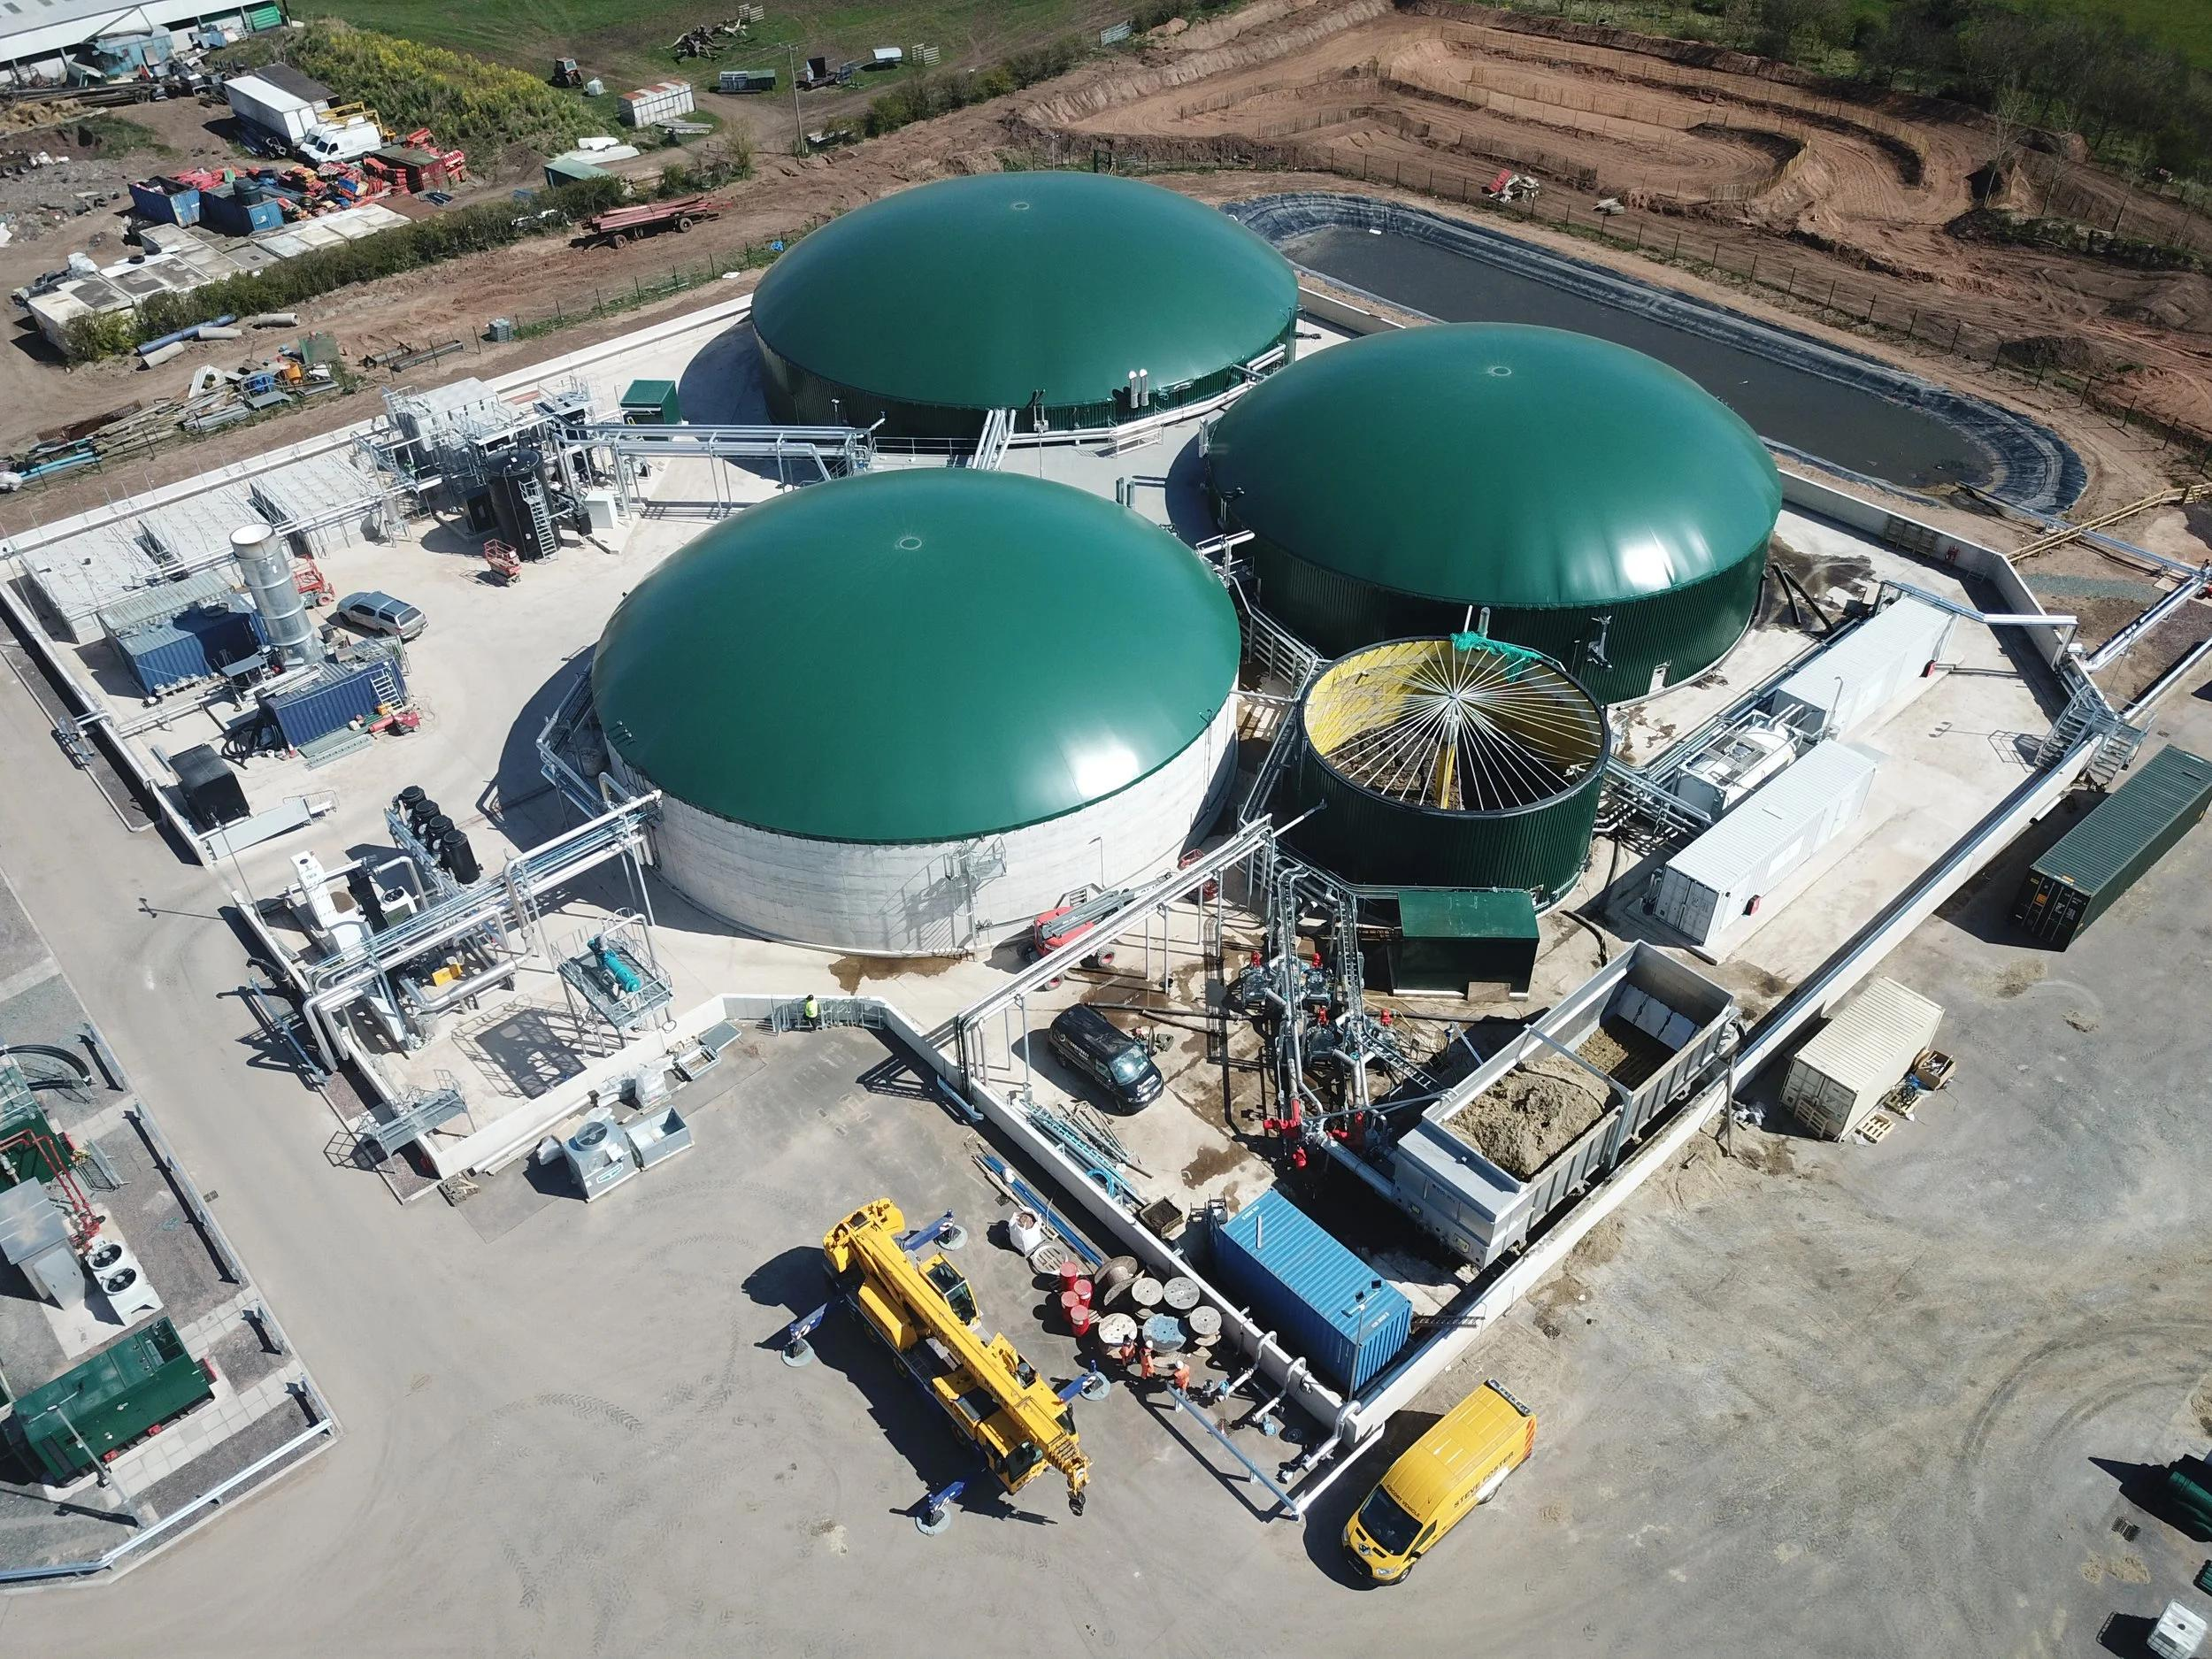
\includegraphics[width=0.8\textwidth]{Figuras/Sección B - Tecnologías de Conversión/Digestores anaeróbicos industriales.jpg}
    \caption{Instalación industrial compuesta por digestores de gran volumen, donde la materia orgánica permanece en condiciones anaeróbicas para favorecer la actividad de los microorganismos metanogénicos. Estos reactores permiten procesar grandes cantidades de residuos orgánicos y producir biogás de manera continua}
\end{figure}

Antes de alimentar motores o inyectarse a red, el biogás se seca y desulfura (para remover el $\mathrm{H_2S}$ corrosivo y siloxanos en gas de relleno). Mediante separación de $\mathrm{CO_2}$ (lavado con agua, PSA o membranas) se obtiene \textit{biometano} ($>95~\%~\mathrm{CH_4}$). La IEA estima un potencial global sostenible cercano a $10^{12}~\text{m}^3$ equivalentes de gas natural al año, del cual hoy se aprovecha menos del 5~\% (1,76~EJ en 2023) \cite{iea2025biogas, wba2025gbsr}.

\section{Comparación de rutas para generación eléctrica}
\label{sec:comparacion_rutas}

La Tabla~\ref{tab:comparacion_rutas} sintetiza el desempeño eléctrico, la escala típica y la madurez comercial de las distintas tecnologías analizadas. No existe una opción universalmente superior: la combustión con ciclo Rankine domina en mediana y gran escala con biomasa sólida; la gasificación y el ORC atienden nichos descentralizados; y la digestión anaeróbica con motogeneradores lidera en residuos húmedos.

\begin{table}[H]
\centering
\caption{Comparación de sistemas de generación eléctrica con biomasa (valores orientativos).}
\label{tab:comparacion_rutas}
\begin{tabularx}{\textwidth}{@{}X l l l@{}}
\toprule
\textbf{Sistema de generación} & \textbf{Escala típica} & \textbf{$\eta$ eléctrica} & \textbf{Madurez} \\
\midrule
Caldera + turbina de vapor (Rankine), dedicada & 5--300~$\mathrm{MW_e}$ & 20--35~\% & Comercial madura \\
Co-combustión en central de carbón & $>100~\mathrm{MW_e}$ & 36--44~\% \cite{irena2013cofiring} & Comercial \\
Caldera + ciclo Rankine orgánico (ORC) & 0,2--5~$\mathrm{MW_e}$ & 15--20~\% & Comercial \\
Gasificador + motor de combustión interna & 0,1--pocos $\mathrm{MW_e}$ & 20--30~\% & Comercial (exige limpieza) \\
Gasificación integrada en ciclo combinado (BIGCC) & $>20~\mathrm{MW_e}$ & 35--45~\% (proy.) & Demostración \\
Biogás + motogenerador & 0,05--5~$\mathrm{MW_e}$ & 35--42~\% (s/biogás) & Comercial madura \\
Pirólisis + motor o turbina & --- & --- & Precomercial \\
\bottomrule
\end{tabularx}
\end{table}

\begin{figure}[H]
    \centering
    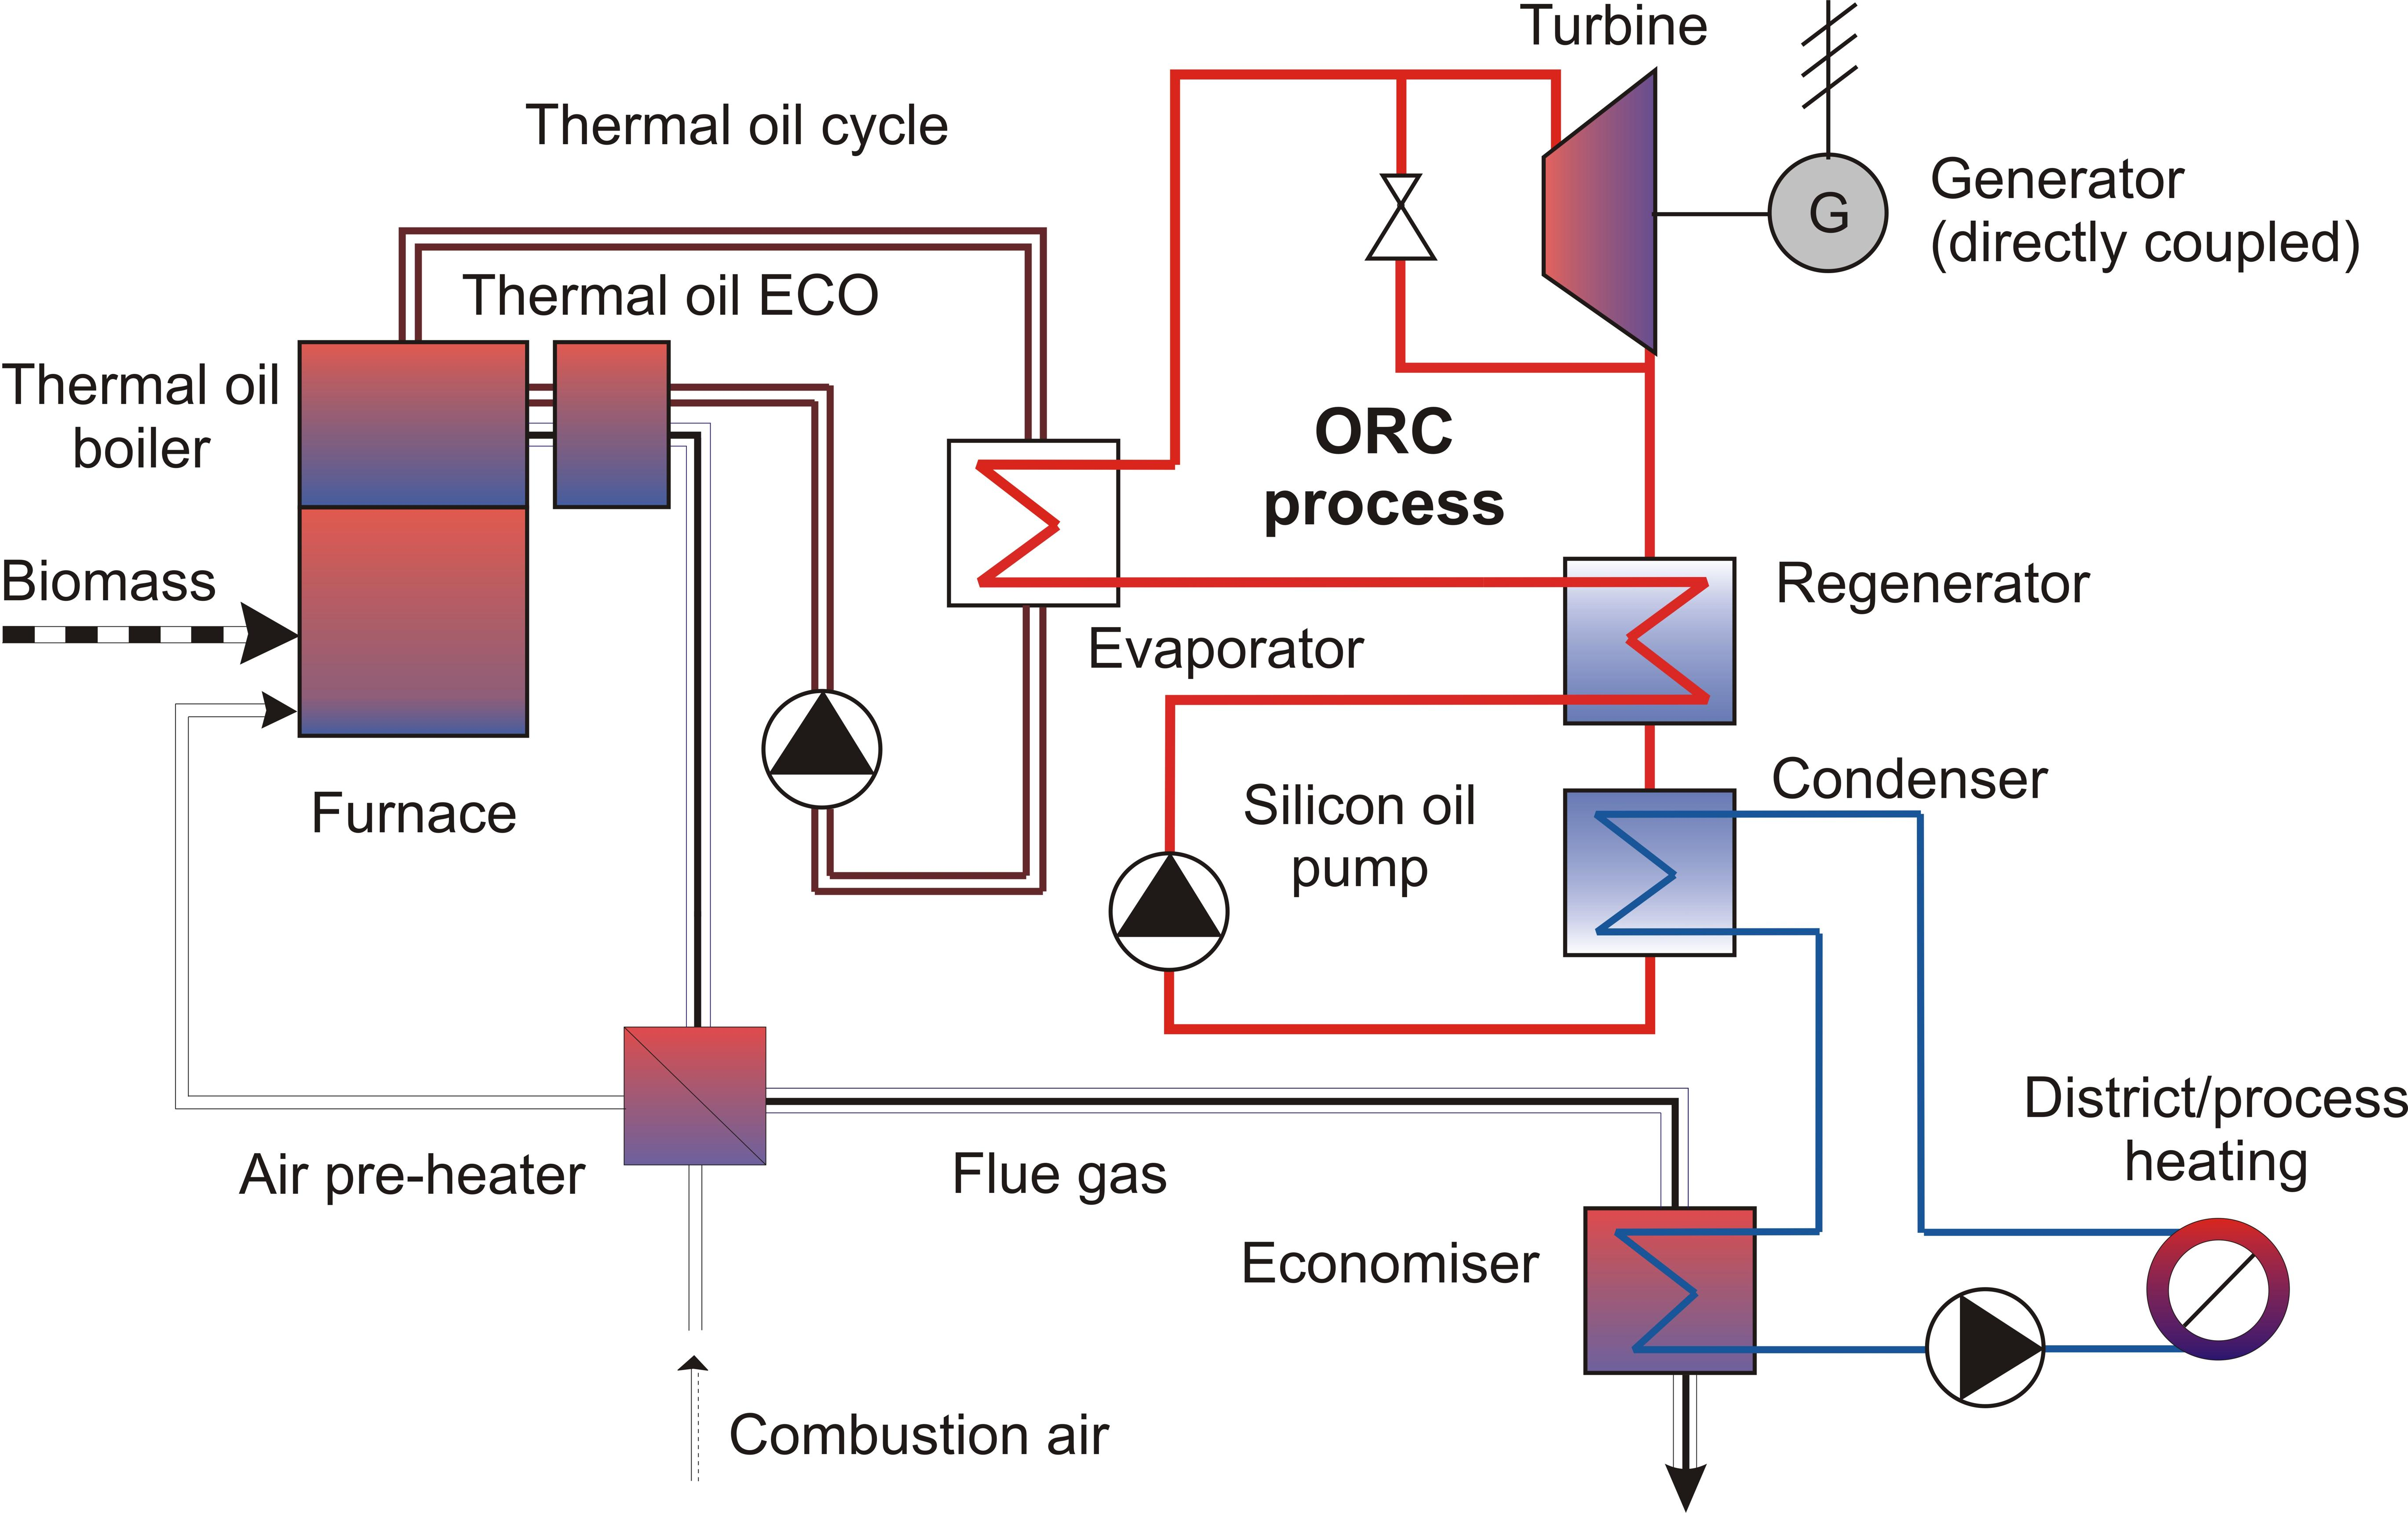
\includegraphics[width=0.9\textwidth]{Figuras/Sección B - Tecnologías de Conversión/Generación eléctrica mediante ciclo Rankine orgánico (ORC).jpg}
    \caption{Generación eléctrica mediante ciclo Rankine orgánico (ORC): El calor procedente de una fuente térmica se transfiere a un fluido orgánico de bajo punto de ebullición. El vapor generado acciona una turbina conectada a un generador eléctrico y posteriormente se condensa para retornar al evaporador, cerrando el ciclo. Esta tecnología permite aprovechar fuentes de calor de temperaturas relativamente bajas}
\end{figure}

\begin{figure}[H]
    \centering
    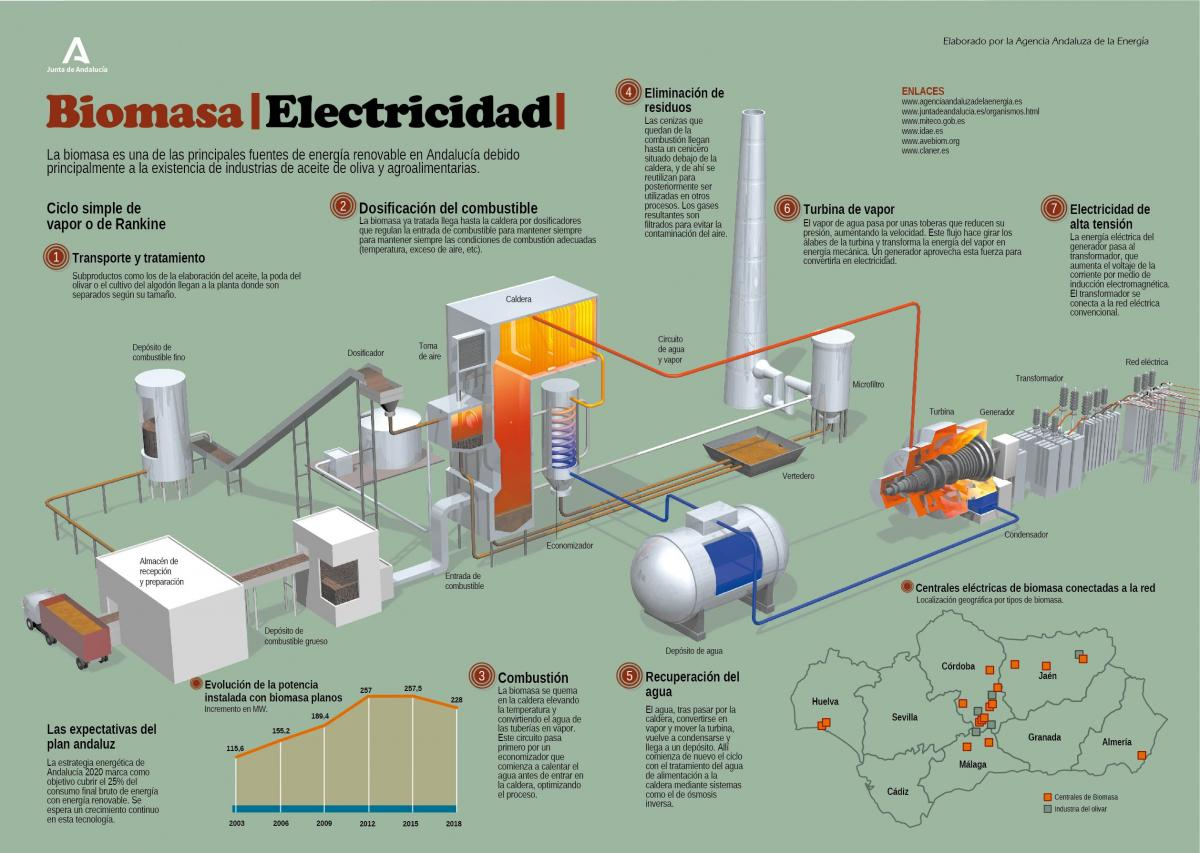
\includegraphics[width=0.75\textwidth]{Figuras/Sección B - Tecnologías de Conversión/Generación eléctrica mediante combustión directa y ciclo Rankine.jpg}
    \caption{Generación eléctrica mediante combustión directa y ciclo Rankine: Sistema de generación eléctrica en el que la biomasa sólida se quema en una caldera para producir vapor de agua a alta presión y temperatura. Este vapor se expande en una turbina acoplada a un generador eléctrico, mientras que posteriormente se condensa y recircula para completar el ciclo termodinámico}
\end{figure}

\begin{figure}[H]
    \centering
    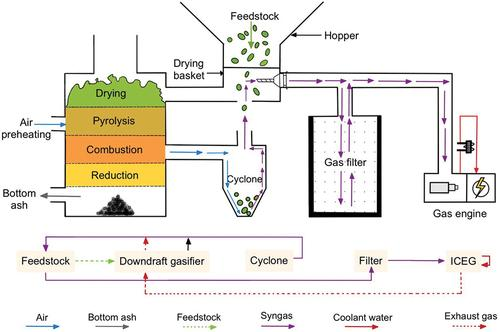
\includegraphics[width=0.75\textwidth]{Figuras/Sección B - Tecnologías de Conversión/Gasificación de biomasa para generación eléctrica.jpg}
    \caption{Gasificación de biomasa para generación eléctrica: Proceso de conversión termoquímica de biomasa sólida en un gas combustible mediante su reacción a temperaturas elevadas con una cantidad controlada de agente gasificante. El gas producido, compuesto principalmente por monóxido de carbono, hidrógeno y metano, pasa por un sistema de acondicionamiento y limpieza antes de alimentar un motor de combustión interna acoplado a un generador eléctrico}
\end{figure}

\begin{figure}[H]
    \centering
    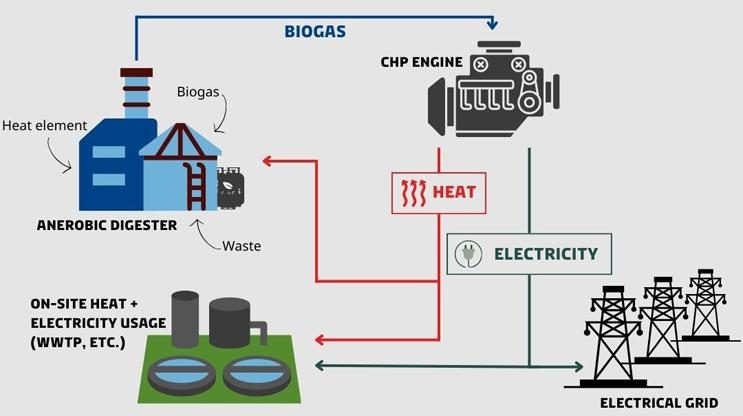
\includegraphics[width=0.8\textwidth]{Figuras/Sección B - Tecnologías de Conversión/Generación eléctrica mediante biogás y ciclo de cogeneración.jpg}
    \caption{Generación eléctrica mediante biogás y ciclo de cogeneración: Utiliza el biogás producido en un digestor anaeróbico como combustible para alimentar un motor de combustión interna acoplado a un generador eléctrico. Además de producir electricidad, el sistema recupera el calor residual de los gases de escape y del circuito de refrigeración del motor para su aprovechamiento térmico, incrementando la eficiencia energética global de la instalación}
\end{figure}

En términos de selección tecnológica, la viabilidad de cada ruta depende principalmente de las características del recurso biomásico, su disponibilidad, contenido de humedad, poder calorífico y escala de aprovechamiento, así como de los requerimientos de inversión y operación. También deben considerarse la eficiencia energética global, los sistemas de pretratamiento y acondicionamiento del combustible y la posibilidad de recuperar el calor residual mediante cogeneración. Por tanto, la elección debe responder a un análisis técnico-económico que contemple tanto el rendimiento de conversión eléctrica como los costos de instalación, mantenimiento, suministro de biomasa y gestión de subproductos. En general, la integración de tecnologías de conversión con sistemas de recuperación energética permite mejorar el aprovechamiento del recurso y reducir las pérdidas, favoreciendo la viabilidad de los proyectos de generación eléctrica a partir de biomasa.

Adicionalmente, el desarrollo de estas tecnologías representa una alternativa para diversificar la matriz energética y reducir la dependencia de los combustibles fósiles, especialmente en regiones con disponibilidad constante de residuos agrícolas, forestales, ganaderos y agroindustriales. Sin embargo, su implementación requiere garantizar un suministro sostenible de materia prima, establecer sistemas eficientes de recolección y transporte y controlar las emisiones generadas durante la conversión. De esta manera, la generación eléctrica con biomasa no solo debe evaluarse por su capacidad de producir energía, sino también por su contribución al aprovechamiento de residuos, la economía circular y la sostenibilidad ambiental a largo plazo.

\chapter{Plantas de biomasa en el mundo}
\label{cap:plantas_mundo}

Este capítulo examina la implementación industrial de las centrales de biomasa a nivel mundial, clasificando sus escalas de potencia y configuraciones constructivas, analizando instalaciones de referencia internacional y regional, y evaluando los servicios eléctricos que aportan a los sistemas de potencia modernos.

\section{Panorama mundial y escalas de planta}
\label{sec:panorama_escalas}

Al cierre de 2025 la capacidad mundial instalada de generación eléctrica con bioenergía alcanzó $154~\text{GW}$, con una adición anual de $3{,}4~\text{GW}$ liderada por Japón ($+1{,}1~\text{GW}$) \cite{irena2026capacity}. En 2024 la producción global de bioelectricidad llegó a $698~\text{TWh}$ \cite{wba2025gbsr}. Asia concentra la mayor parte del crecimiento, habiendo casi triplicado su capacidad en la última década bajo el impulso de China ($209~\text{TWh}$, 30~\% del total mundial), India y Japón; en América destacan Brasil ($58~\text{TWh}$) y Estados Unidos ($47~\text{TWh}$). Por participación porcentual en la matriz eléctrica nacional sobresalen Luxemburgo (30~\%), Uruguay (22~\%) y Estonia (22~\%) \cite{wba2025gbsr}.

En América Latina el combustible predominante es el bagazo de caña de azúcar. Casi el 20~\% de la capacidad mundial de biomasa utiliza bagazo, con Brasil como principal productor seguido por Centroamérica y el Caribe, donde Guatemala concentra cerca de la mitad de la potencia regional \cite{er2019centroamerica, torijano2025cepal}.

Aunque no existe una norma internacional única para definir las escalas de potencia, en ingeniería resulta útil distinguir tres rangos orientativos (Tabla~\ref{tab:escalas_planta}), ya que cada escala se asocia a una tecnología característica.

\begin{table}[htbp]
\centering
\small
\caption{Escalas orientativas de plantas de generación eléctrica con biomasa.}
\label{tab:escalas_planta}
\begin{tabularx}{\textwidth}{@{}p{1.4cm} p{1.7cm} X X p{3.0cm}@{}}
\toprule
\textbf{Escala} & \textbf{Rango} & \textbf{Tecnologías típicas} & \textbf{Aplicación} & \textbf{Caso de referencia} \\
\midrule
Pequeña & $<1~\mathrm{MW_e}$ & Biodigestor + motogenerador; gasificador \textit{downdraft} + motor; ORC pequeño & Granjas, comunidades aisladas, pequeña agroindustria & Biodigestores en granjas porcinas y lecheras \\
Mediana & $1\text{--}50~\mathrm{MW_e}$ & Caldera de parrilla o BFB + turbina de vapor; ORC; CHP industrial & Ingenios, aserraderos, papeleras, redes térmicas & Ingenios de Guatemala (933~MW en conjunto) \cite{eyn2019guatemala} \\
Grande & $>50~\mathrm{MW_e}$ & Caldera CFB, combustión pulverizada, conversión de carbón & Mercado mayorista; gran cogeneración & Alholmens Kraft ($\sim 265~\mathrm{MW_e}$) \cite{alholmenskraft}; Drax ($4 \times 660$~MW) \cite{drax2025annual} \\
\bottomrule
\end{tabularx}
\end{table}

\subsection{Casos de referencia internacional y regional}
\begin{itemize}[leftmargin=1.5em]
\item \textbf{Mediana escala --- Ingenios azucareros de Guatemala:} La capacidad instalada conjunta de los ingenios guatemaltecos alcanzó $933~\text{MW}$ en 2019 ---más del doble de la mayor hidroeléctrica del país (Chixoy)---, llegando a cubrir hasta el 31~\% de la demanda eléctrica nacional durante la zafra (noviembre a mayo) \cite{eyn2019guatemala}. Mediante mejoras de presión y temperatura de vapor pasaron de generar $44$ a $91~\text{kWh}$ por tonelada de caña molida \cite{er2018bagazo}, logrando además entregar energía al sistema fuera de zafra \cite{prensalatina2024guatemala}.
    \begin{figure}[H]
        \centering
        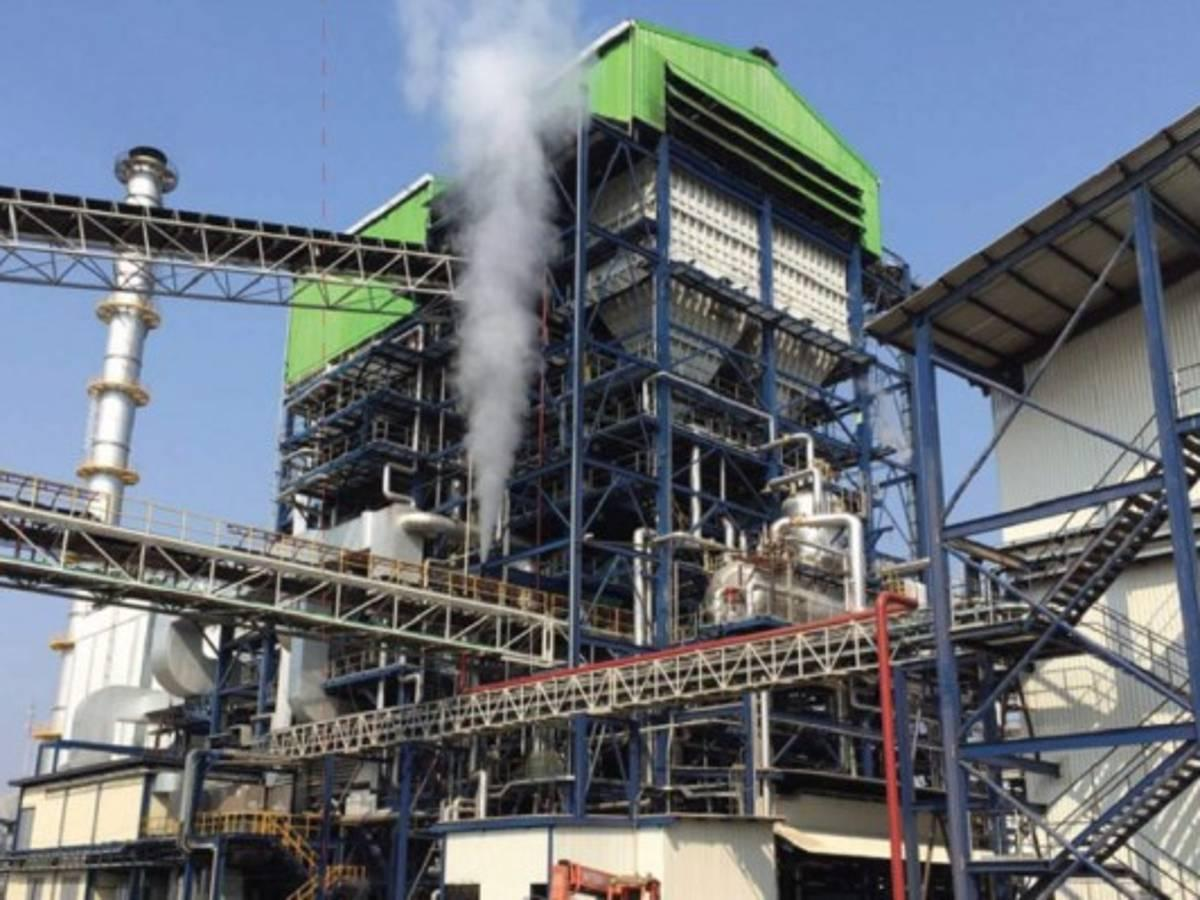
\includegraphics[width=0.9\textwidth]{Figuras/Sección C - Plantas de biomasa por el mundo/Planta de generación eléctrica del Ingenio Magdalena (Guatemala).jpg}
        \caption{Instalación industrial de generación eléctrica del Grupo Magdalena, en Guatemala. Se observan estructuras de calderas, tuberías, plataformas y equipos auxiliares empleados en la conversión térmica para producir electricidad. Es un ejemplo de infraestructura de generación energética vinculada a la industria azucarera guatemalteca}
    \end{figure}
\item \textbf{Gran escala --- Alholmens Kraft (Finlandia):} Considerada la mayor central de cogeneración con biomasa del mundo. Cuenta con $\sim 265~\mathrm{MW_e}$ instalados y una caldera de lecho fluidizado circulante (CFB) de $500~\mathrm{MW_{th}}$ a $165~\text{bar}$ y $545$~\textdegree C, suministrando además $100~\mathrm{MW_{th}}$ de vapor de proceso a una industria papelera vecina y $60~\mathrm{MW_{th}}$ de calefacción urbana a Pietarsaari \cite{alholmenskraft, flynn2005alholmens}. Fue diseñada como planta multicombustible (residuos forestales, turba y carbón); de sus 400 empleados, alrededor de 350 trabajan en la cadena de producción y manejo del combustible.
\item \textbf{Gran escala --- Drax Power Station (Reino Unido):} Originalmente la mayor central de carbón británica con seis unidades de $660~\text{MW}$. Entre 2013 y 2018 reconvirtió cuatro unidades para quemar exclusivamente pellets de madera ($\sim 2{,}6~\text{GW}$ totales), cerrando las dos unidades de carbón restantes en 2021 \cite{drax2025annual}. En 2024 generó más del 5~\% de la electricidad del Reino Unido, importando millones de toneladas anuales de pellets desde Norteamérica, lo que ilustra tanto la viabilidad de reutilizar infraestructura térmica como los límites logísticos de la gran escala.
\end{itemize}

\begin{figure}[H]
    \centering
    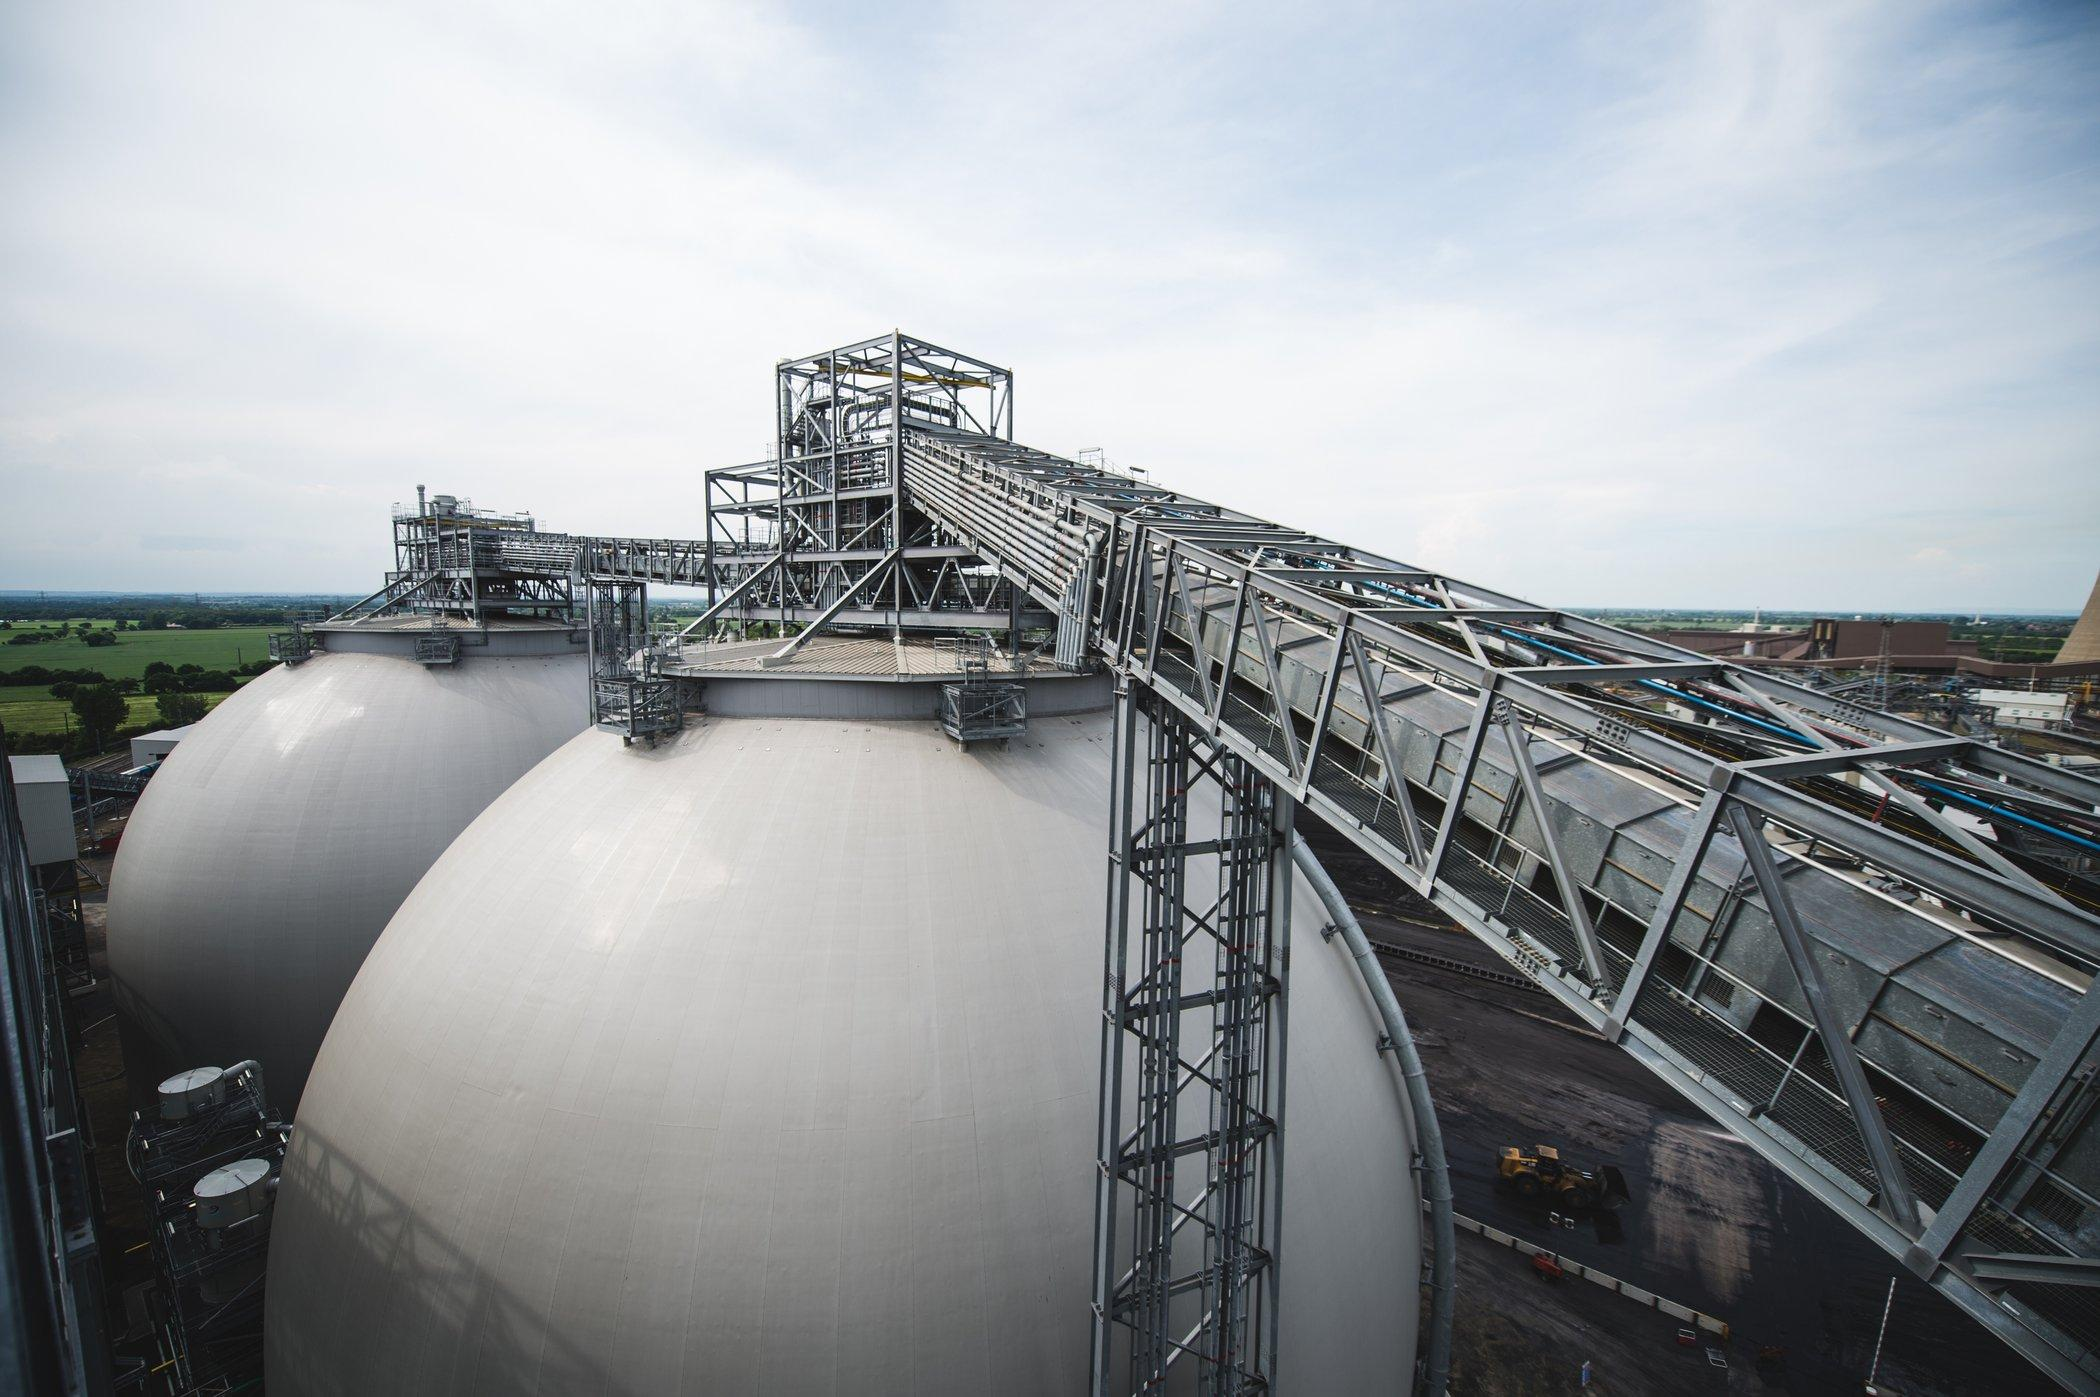
\includegraphics[width=0.75\textwidth]{Figuras/Sección C - Plantas de biomasa por el mundo/Sistema de almacenamiento de pellets de madera de Drax (Reino Unido).jpg}
    \caption{Grandes estructuras abovedadas utilizadas para almacenar pellets de madera en la central Drax. Estas instalaciones permiten mantener reservas de combustible para garantizar el suministro continuo a las unidades de generación, independientemente de las variaciones en las entregas de biomasa}
\end{figure}

\begin{figure}[H]
    \centering
    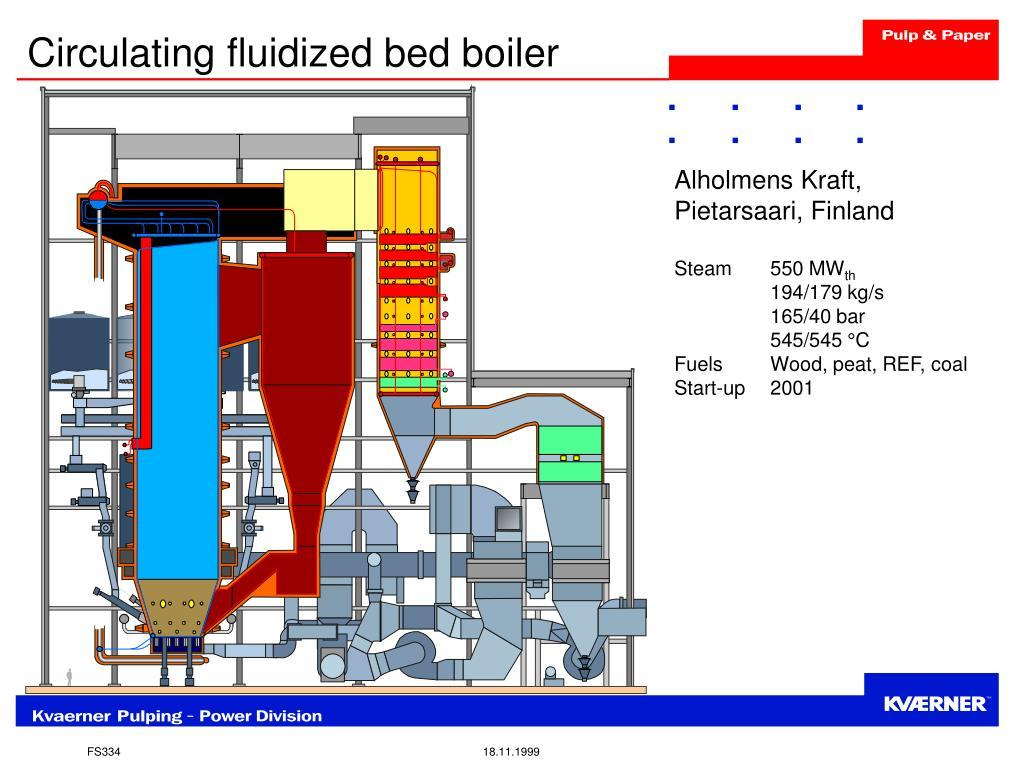
\includegraphics[width=0.7\textwidth]{Figuras/Sección C - Plantas de biomasa por el mundo/Caldera de lecho fluidizado circulante (CFB) de Alholmens Kraft.jpg}
    \caption{Esquema constructivo de una caldera de lecho fluidizado circulante utilizada en la central Alholmens Kraft, Finlandia. Se identifican la cámara de combustión, los sistemas de circulación de sólidos, los separadores ciclónicos y las superficies de intercambio térmico. Esta tecnología permite aprovechar diferentes combustibles sólidos y mantener condiciones de combustión controladas para producir vapor a alta presión y temperatura}
\end{figure}

\section{Configuraciones de planta}
\label{sec:configuraciones}

Según el aprovechamiento térmico y la integración con centrales existentes, se distinguen cuatro configuraciones principales (Tabla~\ref{tab:configuraciones_planta}). La \textbf{cogeneración (CHP)} es la configuración que mejor rentabiliza un combustible costoso de transportar, al elevar la eficiencia energética global al 70--90~\% mediante la venta o uso simultáneo de electricidad y vapor útil; esto exige ubicar la central junto al consumidor térmico (ingenios, papeleras, aserraderos o redes de distrito).

\begin{table}[htbp]
\centering
\caption{Configuraciones constructivas de centrales de biomasa.}
\label{tab:configuraciones_planta}
\begin{tabularx}{\textwidth}{@{}l X l l@{}}
\toprule
\textbf{Configuración} & \textbf{Descripción} & \textbf{Eficiencia típica} & \textbf{Ejemplo} \\
\midrule
Planta dedicada & Solo electricidad mediante turbina de condensación. & 20--35~\% eléctrica & Centrales forestales \\
Cogeneración (CHP) & Electricidad y calor útil del mismo combustible (contrapresión o extracción). & 70--90~\% global & Alholmens; ingenios \\
Co-combustión & Biomasa mezclada con carbón en caldera existente. & 36--44~\% eléctrica \cite{irena2013cofiring} & Centrales europeas \\
Conversión total & Central de carbón adaptada para operar 100~\% con biomasa. & Similar a la original & Drax \cite{drax2025annual} \\
\bottomrule
\end{tabularx}
\end{table}

\section{Aporte al sistema de potencia}
\label{sec:aporte_red}

A medida que crece la penetración de generación solar fotovoltaica y eólica ---recursos variables conectados a la red mediante inversores electrónicos---, los sistemas eléctricos demandan no solo energía, sino también potencia firme, flexibilidad operativa, inercia física y control de frecuencia y tensión \cite{bindu2025inertia, denholm2020inertia}. Una central de biomasa equipada con turbina y generador síncrono aporta estos servicios de estabilidad de manera natural, de forma equivalente a una central térmica convencional pero con combustible renovable.

\subsection{Potencia firme y reserva rodante}
Debido a que la biomasa se almacena en patios de astillas, silos de pellets o gasómetros, la generación puede programarse según la curva de demanda y no según la meteorología, explicando el factor de planta mundial medio de $\sim 53~\%$ \cite{wba2025gbsr}. En el Reino Unido, Drax suscribió un contrato por diferencia (CfD) como generación despachable baja en carbono a partir de abril de 2027 \cite{woodbioenergy2026drax}, y la IEA destaca el rol del biogás para el balance de red \cite{iea2025biogas}. La principal restricción es la estacionalidad de ciertos residuos agroindustriales como el bagazo.

En cuanto a la \textbf{reserva rodante}, las unidades sincronizadas que operan por debajo de su potencia nominal pueden incrementar carga ante la salida intempestiva de otro generador. En plantas de vapor, la velocidad de respuesta está limitada por la inercia térmica de la caldera (más lenta que en turbinas de gas o hidroeléctricas), mientras que los motogeneradores a biogás responden en minutos.

\subsection{Inercia rotacional y regulación primaria de frecuencia}
La inercia física corresponde a la energía cinética almacenada en las masas rotantes (turbina y rotor del generador síncrono) acopladas electromagnéticamente a la red \cite{nrel2014inertia, denholm2020inertia}. Ante la pérdida súbita de un generador ($\Delta P$), las masas rotantes liberan energía instantáneamente, frenando la caída de frecuencia y dando margen de actuación a los reguladores de velocidad. Se cuantifica mediante la constante de inercia $H$:
\begin{equation}
E_{\mathrm{cin}} = \frac{1}{2} J \omega^2, \qquad H = \frac{E_{\mathrm{cin}}}{S_n} \quad [\text{s}]
\end{equation}
donde $S_n$ es la potencia aparente nominal. La tasa inicial de cambio de frecuencia (\textit{Rate of Change of Frequency}, RoCoF) tras un desbalance $\Delta P$ resulta aproximadamente:
\begin{equation}
\frac{\mathrm{d}f}{\mathrm{d}t} \approx -\frac{\Delta P}{S_n} \cdot \frac{f_0}{2H}
\end{equation}
En un sistema de $60~\text{Hz}$ que pierde súbitamente el 5~\% de su generación ($\Delta P / S_n = 0{,}05$), con una inercia alta ($H = 4~\text{s}$) el RoCoF inicial es $\approx 0{,}38~\text{Hz/s}$; en cambio, en una red con alta penetración de inversores y baja inercia ($H = 2~\text{s}$), el RoCoF se duplica a $\approx 0{,}75~\text{Hz/s}$, pudiendo activar prematuramente los esquemas de deslastre de carga. Si bien los inversores modernos \textit{grid-forming} pueden emular inercia sintética, la inercia de los generadores síncronos de biomasa es intrínseca y madura.

Tras la respuesta inercial actúa la \textbf{regulación primaria}: el gobernador de la turbina ajusta la admisión de vapor según su estatismo $R$ (\textit{droop}, típicamente 4--5~\%):
\begin{equation}
\frac{\Delta P}{P_n} = -\frac{\Delta f / f_0}{R}
\end{equation}
Así, una unidad de biomasa de $30~\text{MW}$ con $R = 5~\%$ ($0{,}05$) ante una caída de frecuencia de $0{,}3~\text{Hz}$ ($0{,}5~\%$ de $60~\text{Hz}$) incrementa su potencia en $\Delta P = (0{,}005 / 0{,}05) \times 30~\text{MW} = 3~\text{MW}$. Posteriormente intervienen la regulación secundaria (AGC, en minutos) y la terciaria (redespacho).

\subsection{Control de tensión, potencia reactiva y filosofía de control}
Mediante su sistema de excitación y regulador automático de tensión (AVR), el generador síncrono inyecta o absorbe potencia reactiva dentro de su curva de capabilidad, sosteniendo el perfil de tensión en el punto de conexión. Esto resulta especialmente valioso porque muchas centrales de biomasa (ingenios, aserraderos) se ubican en zonas rurales al final de líneas largas de distribución o subtransmisión, donde la red es débil. Adicionalmente, aportan corriente de cortocircuito necesaria para la coordinación de protecciones.

Operativamente, las calderas de parrilla y lecho fluidizado presentan cargas mínimas técnicas del 30--50~\% nominal, rampas de pocos puntos porcentuales por minuto y arranques en frío de varias horas; los lechos fluidizados ofrecen una respuesta más suave por su gran masa térmica de arena. En el control de la central se distinguen dos filosofías: en el modo \textit{turbina sigue a caldera}, la válvula de admisión regula presión y la potencia sigue lentamente a la combustión (estable pero lento); en el modo \textit{caldera sigue a turbina}, la válvula responde de inmediato a la demanda aprovechando el vapor almacenado en el domo, permitiendo cumplir con la regulación primaria. Las centrales modernas emplean un control coordinado que combina ambos esquemas.

\begin{figure}[H]
    \centering
    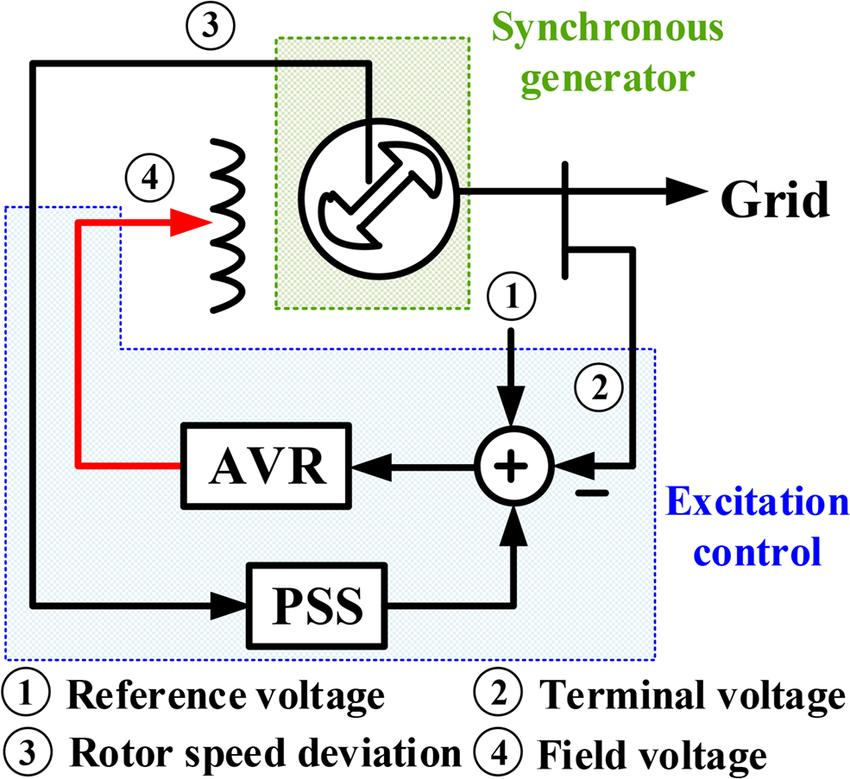
\includegraphics[width=0.98\textwidth]{Figuras/Sección C - Plantas de biomasa por el mundo/Sistema de excitación y regulación de tensión de un generador síncrono (AVR).jpg}
    \caption{Diagrama funcional del sistema de excitación de un generador síncrono, en el que se representa el regulador automático de tensión (AVR) y el estabilizador del sistema de potencia (PSS). El AVR compara la tensión de referencia con la tensión terminal del generador y ajusta la corriente de excitación para mantener el nivel de tensión requerido. El PSS contribuye a amortiguar las oscilaciones electromecánicas y mejorar la estabilidad del sistema eléctrico}
\end{figure}
\chapter{Economía, emisiones y contexto de Panamá}
\label{cap:economia_panama}

La viabilidad integral de una central de biomasa no depende únicamente de la eficiencia termodinámica de sus equipos, sino también del costo del suministro de combustible, la estructura de inversión, las emisiones de ciclo de vida y el marco regulatorio y energético local.

\section{Economía de la generación con biomasa}
\label{sec:economia}

A diferencia de la energía solar fotovoltaica y la eólica ---cuyos costos nivelados se redujeron drásticamente desde 2010 al no requerir combustible---, el costo de generación de la bioenergía ha permanecido prácticamente estable y presenta una alta sensibilidad al precio y logística de la materia prima \cite{irena2025costs}. Para comparar proyectos se utiliza el \textbf{costo nivelado de la electricidad} (LCOE), definido como el costo promedio por unidad de energía eléctrica neta generada durante la vida útil $N$ de la central, descontado a una tasa $r$:
\begin{equation}
\mathrm{LCOE} = \frac{\sum_{t=0}^{N} \dfrac{I_t + \mathrm{O\&M}_t + C_{\mathrm{comb},t}}{(1+r)^t}}{\sum_{t=1}^{N} \dfrac{E_{\mathrm{neta},t}}{(1+r)^t}}
\end{equation}
donde $I_t$ representa las inversiones de capital, $\mathrm{O\&M}_t$ los costos de operación y mantenimiento, $C_{\mathrm{comb},t}$ el gasto en combustible y logística, y $E_{\mathrm{neta},t}$ la electricidad neta entregada a la red tras descontar los consumos auxiliares. Asimismo, la rentabilidad depende críticamente del \textbf{factor de capacidad} ($\mathrm{FC} = E_{\mathrm{anual}} / (P_{\mathrm{nom}} \cdot 8\,760)$), ya que un suministro continuo de combustible permite amortizar la inversión sobre una mayor producción anual.

\begin{table}[htbp]
\centering
\caption{Costos promedio mundiales ponderados de bioenergía para generación eléctrica (plantas nuevas) según IRENA \cite{irena2025costs}.}
\label{tab:costos_irena}
\begin{tabular}{@{}lccc@{}}
\toprule
\textbf{Indicador} & \textbf{2010} & \textbf{2024} & \textbf{Variación} \\
\midrule
Costo total instalado (USD/kW) & 3\,082 & 3\,242 & $+5~\%$ \\
Factor de planta promedio & 72~\% & 73~\% & $+1~\%$ \\
LCOE promedio (USD/kWh) & 0,086 & 0,087 & $+1~\%$ \\
\bottomrule
\end{tabular}
\end{table}

Según IRENA (Tabla~\ref{tab:costos_irena}), en 2024 el LCOE promedio ponderado de la bioenergía fue de $0{,}087~\text{USD/kWh}$, prácticamente igual al de 2010 ($0{,}086~\text{USD/kWh}$), habiendo aumentado un 13~\% respecto a 2023 debido a la volatilidad en los costos del combustible y transporte \cite{irena2025costs}. Como referencia comparativa, IRENA estima el LCOE promedio del carbón en $0{,}073~\text{USD/kWh}$ y el del gas natural en ciclo combinado en $0{,}085~\text{USD/kWh}$. El elevado factor de planta de las centrales nuevas (73~\%) confirma su papel como generación firme.

\begin{figure}[H]
    \centering
    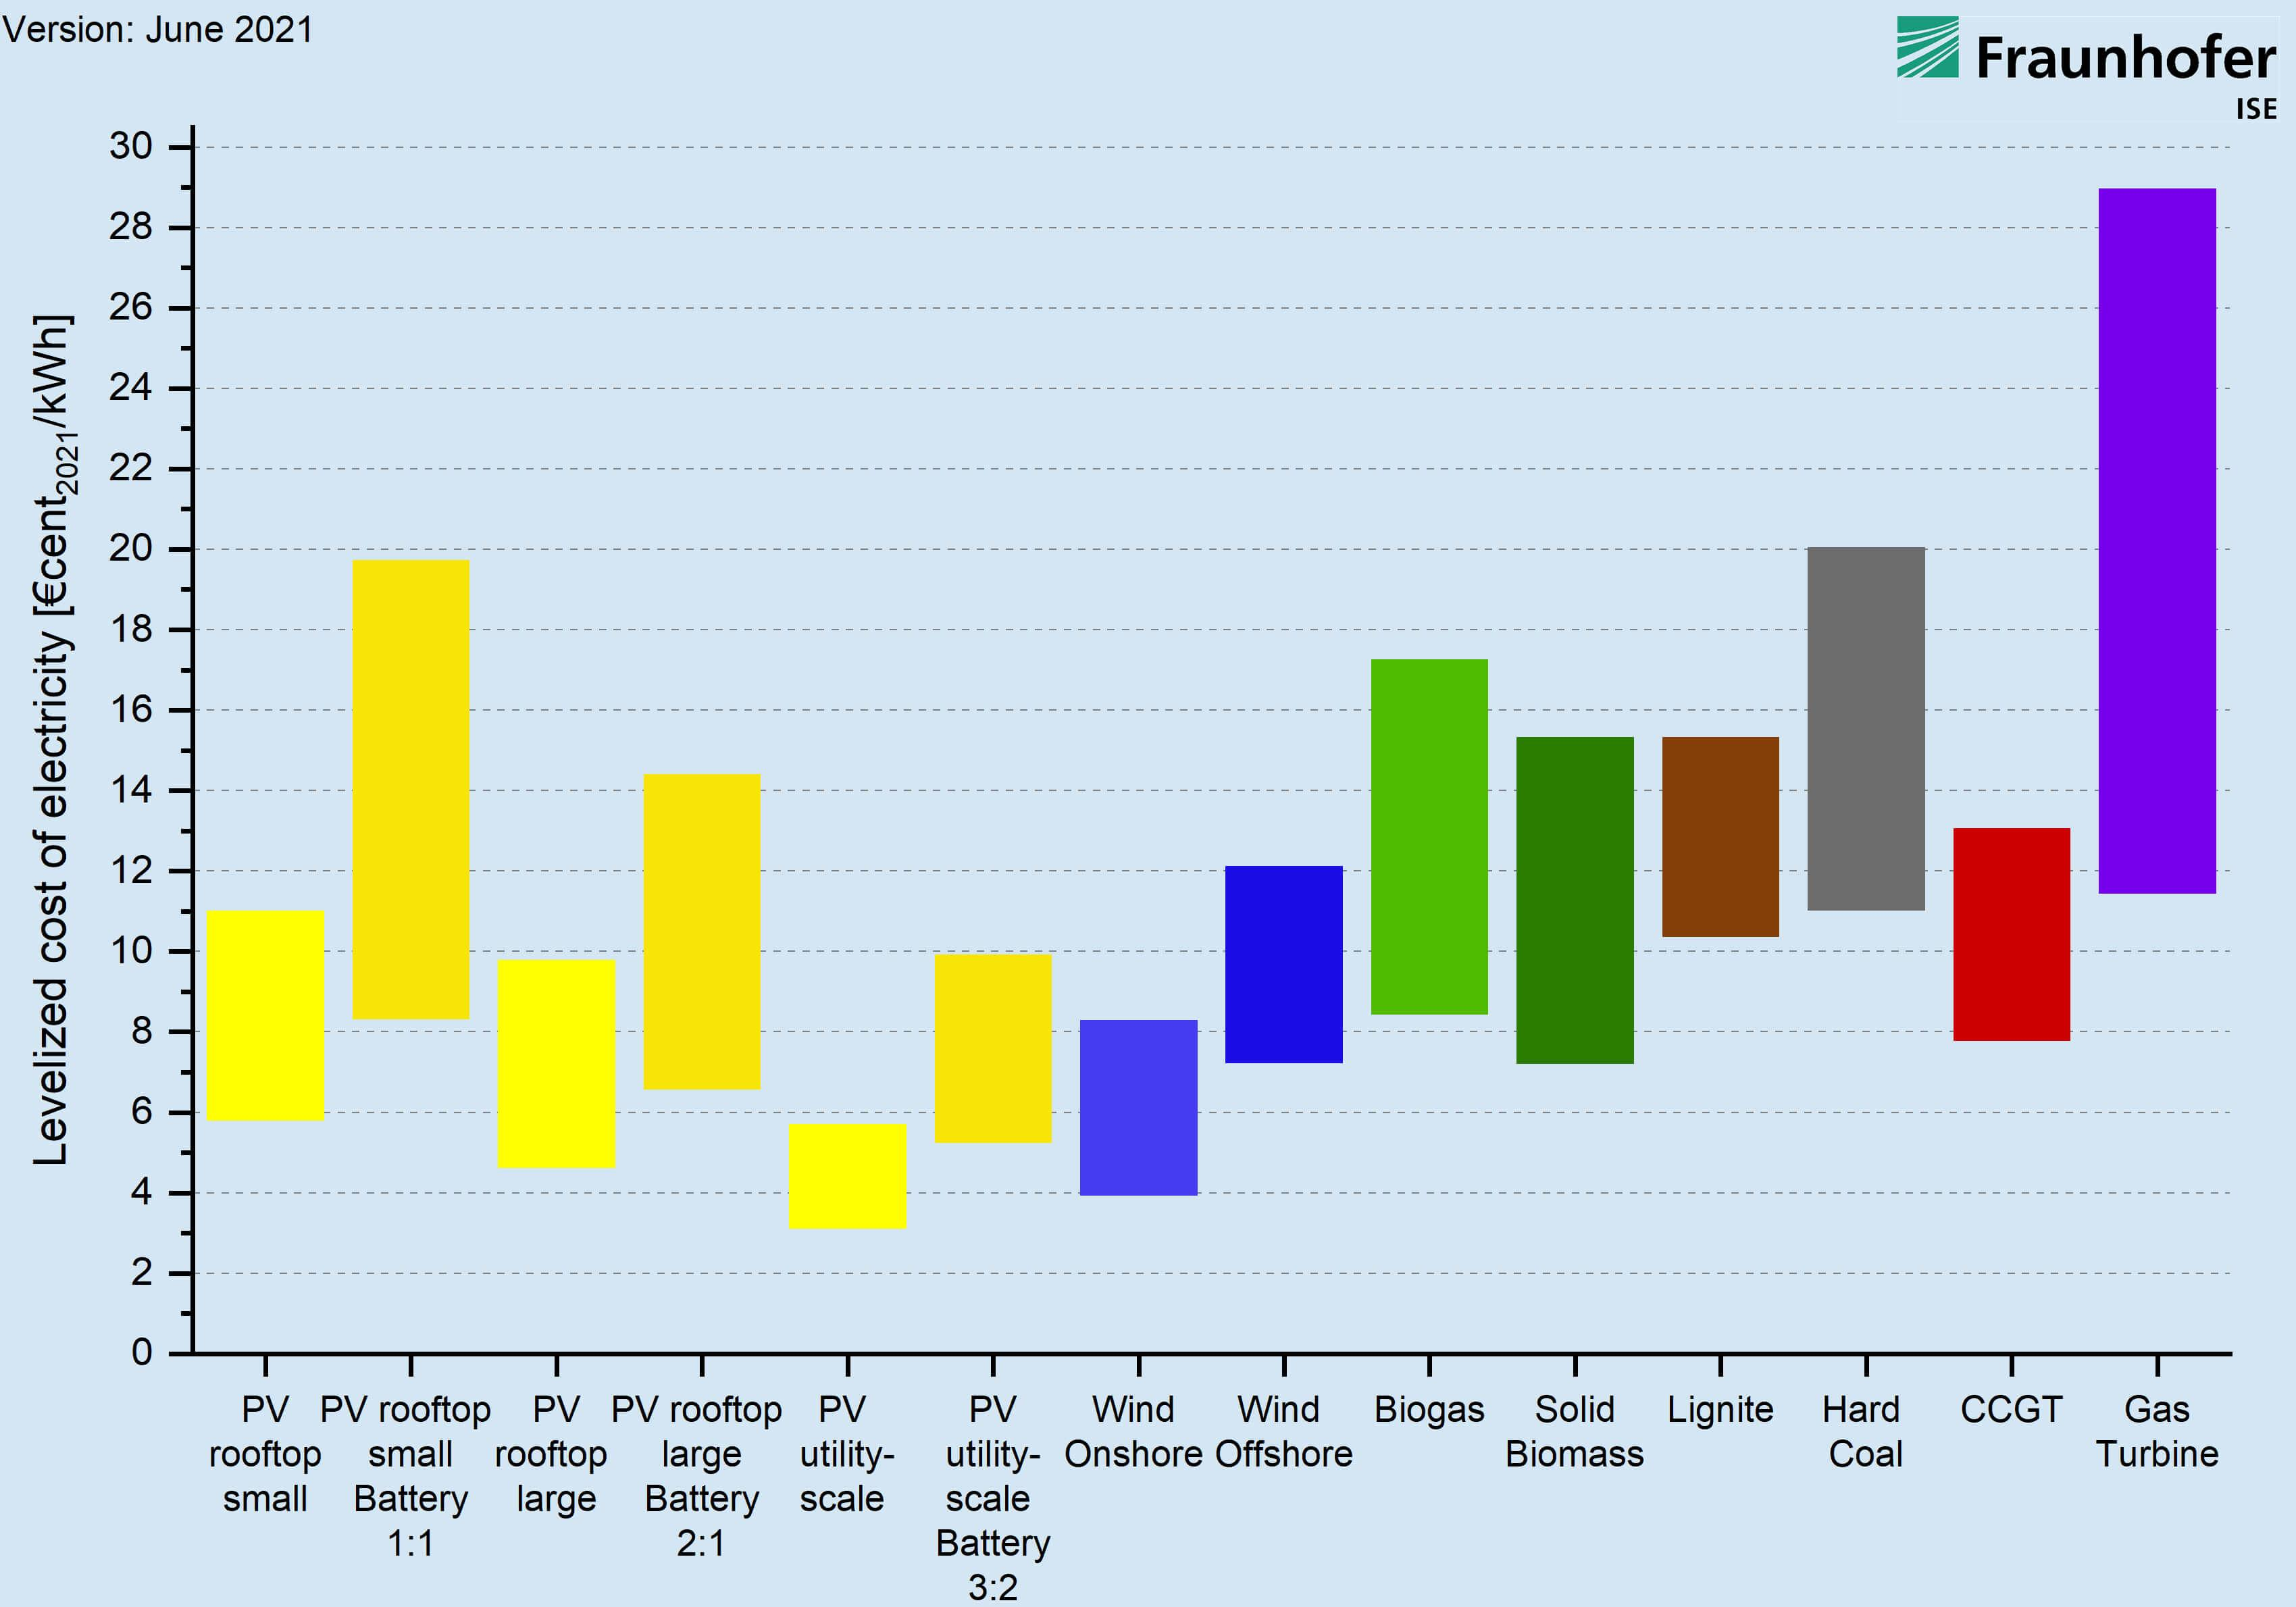
\includegraphics[width=0.7\textwidth]{Figuras/Sección D - Economía, emisiones y contexto de Panamá/Comparación del costo nivelado de electricidad (LCOE) de di.jpg}
    \caption{Gráfica elaborada por el Instituto Fraunhofer ISE que compara los rangos de costos nivelados de electricidad de distintas tecnologías renovables y convencionales, incluyendo biogás y biomasa sólida. Permite visualizar las diferencias económicas entre las alternativas de generación y contextualizar la influencia de los costos de inversión, operación y combustible sobre la competitividad de la bioenergía.}
\end{figure}

La clave económica de un proyecto de biomasa reside en el costo del combustible: al ser un costo variable ausente en la solar o eólica, las centrales más rentables son aquellas que valorizan residuos locales de costo nulo o negativo (bagazo en ingenios, efluentes agroindustriales o residuos que requerirían disposición final) y operan en \textbf{cogeneración}, obteniendo ingresos adicionales por la venta o ahorro de calor de proceso.

\section{Emisiones de ciclo de vida y captura de carbono (BECCS)}
\label{sec:emisiones_beccs}

Aunque el $\mathrm{CO_2}$ emitido en la chimenea de una planta de biomasa es biogénico, el impacto climático real debe evaluarse mediante un \textbf{análisis de ciclo de vida (ACV)} completo. Este contempla las emisiones fósiles de recolección, transporte, secado, peletizado, operación y los cambios directos e indirectos en el uso del suelo \cite{chum2011ipcc, schlomer2014ipcc}. La Tabla~\ref{tab:emisiones_acv} compara las emisiones de ciclo de vida reportadas por el IPCC (2014).

\begin{table}[htbp]
\centering
\caption{Emisiones de ciclo de vida de distintas tecnologías de generación eléctrica en $\text{g CO}_2\text{eq/kWh}$ (IPCC AR5, 2014) \cite{schlomer2014ipcc}.}
\label{tab:emisiones_acv}
\begin{tabular}{@{}lccc@{}}
\toprule
\textbf{Tecnología} & \textbf{Mínimo} & \textbf{Mediana} & \textbf{Máximo} \\
\midrule
Biomasa, planta dedicada & 130 & 230 & 420 \\
Carbón pulverizado & 740 & 820 & 910 \\
Gas en ciclo combinado & 410 & 490 & 650 \\
Solar fotovoltaica (escala de red) & 18 & 48 & 180 \\
Eólica terrestre & 7 & 11 & 56 \\
\bottomrule
\end{tabular}
\end{table}

La generación dedicada con biomasa presenta una mediana de $230~\text{g CO}_2\text{eq/kWh}$ ---alrededor de una cuarta parte del carbón pulverizado ($820~\text{g CO}_2\text{eq/kWh}$) y menos de la mitad del gas en ciclo combinado ($490~\text{g CO}_2\text{eq/kWh}$)---, pero superior a la solar y la eólica. El amplio rango (130--420~$\text{g CO}_2\text{eq/kWh}$) refleja la diferencia entre aprovechar residuos locales frente a utilizar cultivos con cambio de uso del suelo o transporte transoceánico.

Una tecnología emergente es la \textbf{bioenergía con captura y almacenamiento de carbono (BECCS)}, que combina la generación eléctrica con la captura química de $\mathrm{CO_2}$ de los gases de escape, su compresión y su inyección en formaciones geológicas profundas. Si el balance de la cadena de suministro es sostenible, el retiro neto de carbono atmosférico permite alcanzar \textit{emisiones netas negativas}. Como proyecto emblemático, Drax proyecta dos unidades BECCS para capturar $\sim 8~\text{Mt CO}_2/\text{año}$; tras pausarse en 2023, obtuvo aprobación de planificación en 2024 y modificación de permiso ambiental en agosto de 2026, permaneciendo en factibilidad a la espera de un marco de apoyo gubernamental \cite{carbonstorage_drax}. No obstante, la captura de $\mathrm{CO_2}$ impone una penalización energética significativa por regeneración de solventes y compresión, reduciendo la eficiencia eléctrica neta y elevando el LCOE.
\begin{figure}[H]
    \centering
    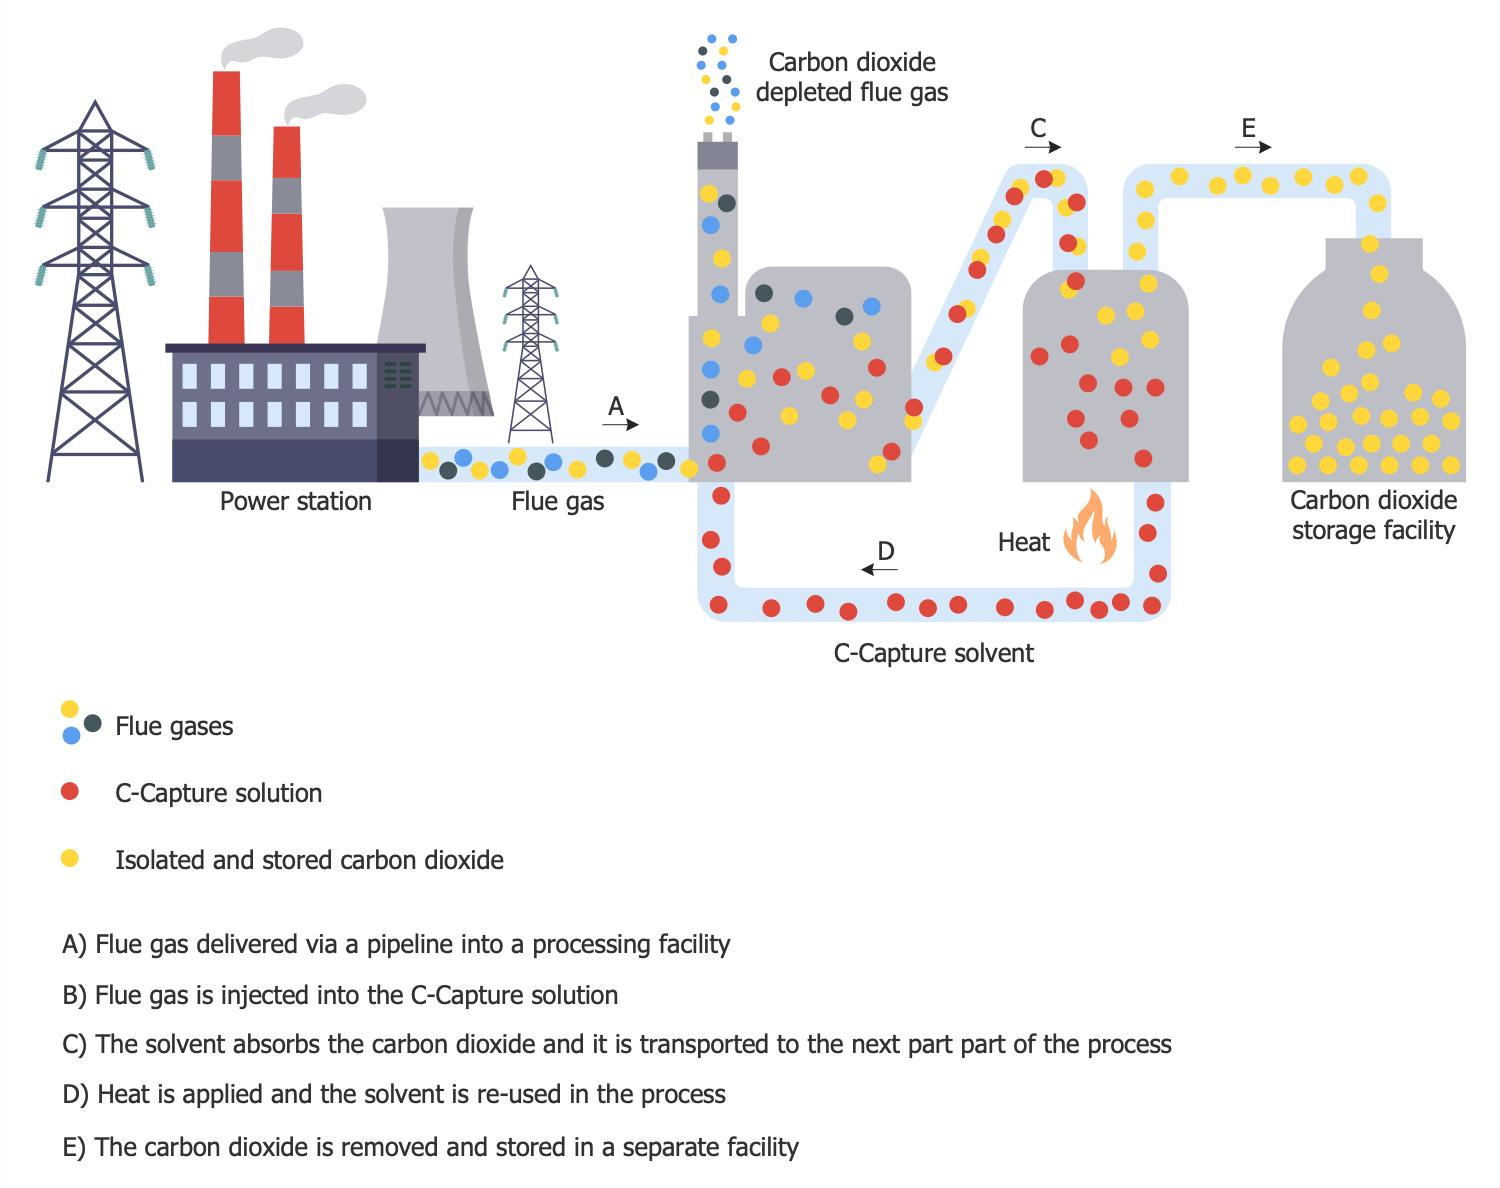
\includegraphics[width=0.8\textwidth]{Figuras/Sección D - Economía, emisiones y contexto de Panamá/Esquema del proceso de captura de.jpg}
    \caption{Diagrama del proceso de captura de dióxido de carbono desarrollado para el proyecto piloto de Drax. Se representa la conducción de los gases de combustión hacia una unidad de tratamiento, donde un solvente químico absorbe el $\mathrm{CO_2}$. Posteriormente, mediante aporte de calor, se regenera el solvente y se separa el dióxido de carbono para su transporte y almacenamiento. Este procedimiento permite ilustrar el principio de funcionamiento de la captura de carbono aplicada a centrales bioenergéticas.}
\end{figure}

\section{Ventajas y limitaciones}
\label{sec:ventajas_limitaciones}

La Tabla~\ref{tab:ventajas_limitaciones} resume el balance técnico, económico y ambiental de la biomasa como tecnología de generación eléctrica.

\begin{table}[htbp]
\centering
\caption{Síntesis de ventajas y limitaciones de la biomasa para generación eléctrica.}
\label{tab:ventajas_limitaciones}
\begin{tabularx}{\textwidth}{@{}X X@{}}
\toprule
\textbf{Ventajas} & \textbf{Limitaciones} \\
\midrule
Renovable y despachable: combustible almacenable que permite generar según demanda. & Costos crecientes: en 2024 el costo instalado subió 16~\% y el LCOE 13~\%, mientras caían otras renovables \cite{irena2025costs}. \\
Valorización de residuos: reduce disposición final y evita emisiones fugitivas de metano en estiércoles y rellenos. & Logística exigente: baja densidad energética, humedad elevada, estacionalidad y dispersión geográfica. \\
Servicios de red: aporta inercia rotacional, regulación primaria de frecuencia y control de tensión. & Riesgos de sostenibilidad: posible deforestación, competencia por suelo/agua y cambio de uso del suelo \cite{chum2011ipcc, fao2016befs}. \\
Alta eficiencia global en cogeneración (70--90~\%) cuando existe demanda térmica cercana. & Emisiones locales: requiere control de material particulado, $\mathrm{CO}$ y $\mathrm{NO}_x$; riesgo de corrosión por cenizas. \\
Generación de empleo rural y local en la cadena de suministro (350 de 400 empleos en Alholmens) \cite{alholmenskraft}. & Posibles fugas de metano en biodigestores mal operados \cite{iea2025biogas} e impactos sociales en monocultivos \cite{er2019centroamerica}. \\
\bottomrule
\end{tabularx}
\end{table}

\section{Contexto de Panamá}
\label{sec:panama}

La matriz eléctrica de Panamá está dominada por la generación hidroeléctrica y térmica convencional, complementadas por solar fotovoltaica y eólica. De acuerdo con las estadísticas de oferta de la Autoridad Nacional de los Servicios Públicos (ASEP) para el segundo semestre de 2025 (Tabla~\ref{tab:asep_panama}), la capacidad instalada total alcanzó $5\,120{,}19~\text{MW}$, sin registrarse plantas dedicadas de biomasa ni de biogás en las estadísticas oficiales de oferta del sistema \cite{asep2025oferta}.

\begin{table}[htbp]
\centering
\caption{Oferta eléctrica de Panamá en 2025 según la ASEP \cite{asep2025oferta}.}
\label{tab:asep_panama}
\begin{tabular}{@{}lccc@{}}
\toprule
\textbf{Tecnología} & \textbf{Capacidad instalada (MW)} & \textbf{Part. en capacidad} & \textbf{Part. en generación 2025} \\
\midrule
Hidroeléctrica & 1\,847,57 & 36,1~\% & 59,8~\% \\
Térmica & 2\,165,97 & 42,3~\% & 25,3~\% \\
Solar fotovoltaica & 770,65 & 15,1~\% & 9,6~\% \\
Eólica & 336,00 & 6,6~\% & 5,3~\% \\
\midrule
\textbf{Total} & \textbf{5\,120,19} & \textbf{100,0~\%} & \textbf{100,0~\%} \\
\bottomrule
\end{tabular}
\end{table}

Registros históricos mostraban una presencia marginal: publicaciones de la UTP citando a la Secretaría Nacional de Energía ubicaban la biomasa en $0{,}24~\%$ de la generación ($8{,}1~\text{MW}$) \cite{utp_pajacanalera}, y en el mercado eléctrico panameño figuran ingenios como autogeneradores o cogeneradores (por ejemplo, Azucarera Nacional S.\,A. registrada ante el Centro Nacional de Despacho), cuya producción se destina principalmente al autoconsumo industrial durante la zafra.

\begin{figure}[H]
    \centering
    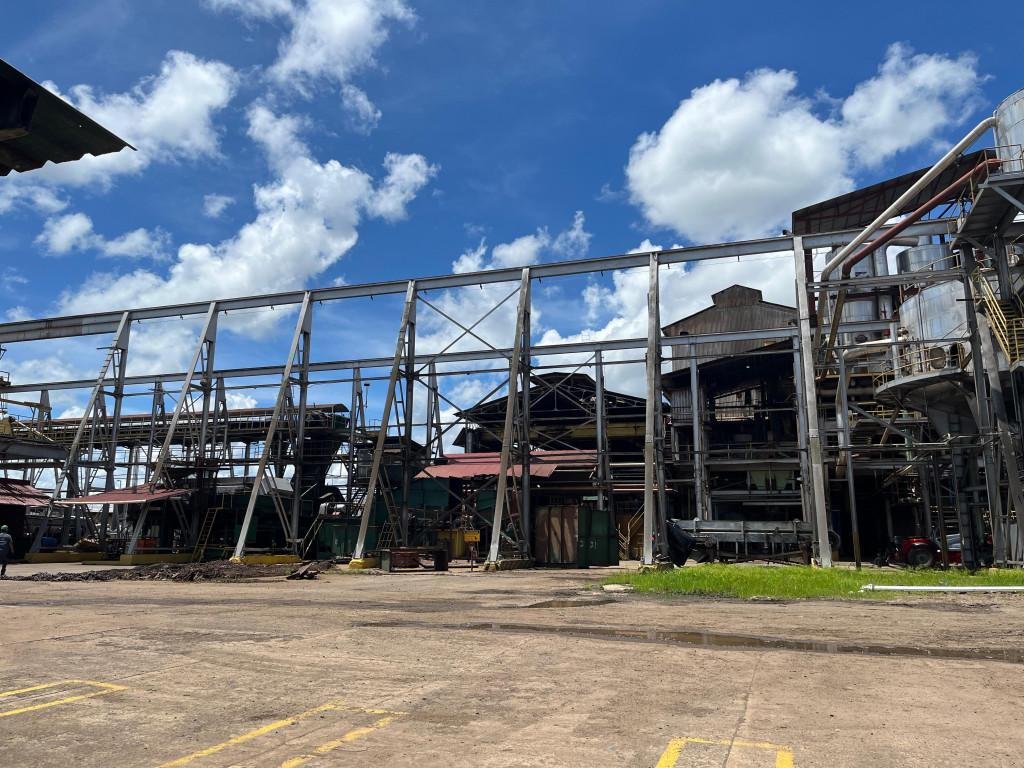
\includegraphics[width=0.75\textwidth]{Figuras/Sección D - Economía, emisiones y contexto de Panamá/Instalaciones industriales del Ingenio Santa Rosa en Panamá.jpg}
    \caption{Fotografía de las instalaciones del Ingenio Santa Rosa, ubicado en El Roble de Aguadulce, provincia de Coclé. Esta instalación representa la infraestructura agroindustrial vinculada al procesamiento de caña de azúcar en Panamá. Su interés energético radica en el aprovechamiento potencial del bagazo como combustible para calderas y sistemas de cogeneración mediante ciclos de vapor.}
\end{figure}

En el plano normativo, el país cuenta con la \textbf{Ley 42 de 20 de abril de 2011}, que establece la política de fomento a los biocombustibles y a la generación y cogeneración eléctrica a partir de biomasa \cite{panama2011ley42}. Asimismo, la elaboración del Plan Energético Nacional 2026--2040 constituye una oportunidad para reevaluar el potencial bioenergético nacional. Entre los recursos identificados con mayor proyección en Panamá destacan:
\begin{itemize}[leftmargin=1.5em]
\item \textbf{Bagazo de caña y residuos del arroz:} concentrados en ingenios azucareros y molinos de las provincias centrales y Chiriquí, aptos para calderas de cogeneración.
\item \textbf{Efluentes porcinos, avícolas y de palma aceitera:} sustratos húmedos idóneos para biodigestores de laguna cubierta o reactores CSTR con motogeneradores.
\item \textbf{Paja canalera (\textit{Saccharum spontaneum}):} especie invasora abundante en la cuenca del Canal cuya caracterización y gasificación han sido investigadas por la Universidad Tecnológica de Panamá \cite{utp_pajacanalera}.
\item \textbf{Biogás de rellenos sanitarios:} particularmente el potencial de captación y valorización energética estudiado en el relleno sanitario de Cerro Patacón \cite{unachi_cerropatacon}.
\end{itemize}
Su aprovechamiento futuro requerirá inventarios confiables de disponibilidad y estacionalidad de residuos, estudios de factibilidad logística y esquemas tarifarios o de contratación adecuados para cogeneración y generación distribuida.


% -------------------------------------------------------------------------
% 5. CONCLUSIONES
% -------------------------------------------------------------------------
\input{Capitulos/06_conclusiones}

% -------------------------------------------------------------------------
% 6. BIBLIOGRAFÍA (ESTILO IEEE)
% -------------------------------------------------------------------------
\clearpage
\addcontentsline{toc}{chapter}{Bibliografía}
\renewcommand{\bibname}{Bibliografía}
\bibliographystyle{IEEEtran}
\bibliography{referencias}

\end{document}
